\documentclass{ieeeaccess}
\usepackage{cite}
\usepackage{amsmath,amssymb,amsfonts}
\usepackage{algorithmic}
\usepackage{graphicx}
\usepackage{textcomp}
\usepackage{booktabs}
\usepackage{url}
\usepackage{multirow}

\def\BibTeX{{\rm B\kern-.05em{\sc i\kern-.025em b}\kern-.08em
    T\kern-.1667em\lower.7ex\hbox{E}\kern-.125emX}}

\begin{document}
\history{Manuscript Draft: October 12, 2026. Prepared for Peer Review.}
\doi{}

\title{An AI-Driven Adaptive Cybersecurity Framework for IoT: Anomaly Detection, Dynamic Thresholding, Un-Contaminated Reinforcement Learning Defense, Post-Quantum Cryptography, and Tamper-Evident Audit Logging}

\author{\uppercase{Tanish Thakare}\authorrefmark{1}}

\address[1]{Department of Computer Science and Engineering, Independent Research (e-mail: tanish.thakare2005@gmail.com)}

\tfootnote{This research was supported by academic computing resources. The complete experimental codebase, deterministic data splitting protocols, and evaluation manifests are openly accessible at \url{https://github.com/Tanish-boop/AI-Driven-IoT-Cybersecurity-Framework-Research-}.}

\markboth
{T. Thakare: An AI-Driven Adaptive Cybersecurity Framework for IoT}
{T. Thakare: An AI-Driven Adaptive Cybersecurity Framework for IoT}

\corresp{Corresponding author: Tanish Thakare (e-mail: tanish.thakare2005@gmail.com).}

\begin{abstract}
In Internet of Things (IoT) edge cybersecurity, deep reconstruction-based autoencoders provide effective detection of zero-day network intrusions without requiring labeled attack samples during training. However, translating continuous reconstruction errors into operational mitigation decisions faces critical vulnerabilities: static decision thresholds explode in false alarms under non-stationary traffic surges, un-guarded adaptive thresholds suffer severe threshold inflation collapse during attack floods, defensive reinforcement learning policies risk evaluation split contamination, and existing literature relies on abstract non-standardized cryptographic assumptions. This paper presents an empirically rigorous benchmark evaluating an integrated five-stage cybersecurity framework on CICIoT2023 across 5 random seeds ($42, 123, 456, 789, 2026$) under strictly isolated training, validation, supervised, and held-out test splits. Our empirical results establish that: (1) Sample-level Dense Autoencoders ($L=1$) eliminate sequence window boundary contamination, achieving an unsupervised baseline F1-Score of $0.8854 \pm 0.0013$ ($\text{FPR} = 4.93 \pm 0.13\%$); (2) Excluded EWMA thresholding prevents inflation collapse, reaching F1 = $0.9014 \pm 0.0018$ and coming within 2.55\% of a supervised XGBoost oracle (F1 = $0.9269 \pm 0.0004$), albeit with a higher false positive rate ($13.60 \pm 1.10\%$); (3) Static 95th percentile thresholds suffer a +454.4\% explosion in false positive rates under $2.0\times$ synthetic rate feature scaling; (4) Under strictly un-contaminated evaluation ($X_{\text{sup}}$ training, held-out $X_{\text{test}}$ evaluation), Deep Q-Networks achieve $71.26 \pm 0.09\%$ attack containment with $0.63 \pm 0.46\%$ false block rate (decision latency: $0.1160 \pm 0.0052$~ms), while Tabular Q-Learning achieves a $0.00\%$ false block rate in isolated testing; (5) Standardized NIST FIPS 203 ML-KEM-768 key encapsulation paired with AES-256-GCM achieves sub-millisecond key establishment ($0.2758$~ms KEM, $0.2905$~ms first-message setup) and 100\% tamper rejection; (6) HMAC-SHA-256 ($0.0470$~ms creation) and Tamper-Evident Hash-Chain Audit Logging ($0.0605$~ms append, $\mathcal{O}(1)$ scaling) provide verifiable sequence integrity and tamper localization; (7) In sensitivity testing, evaluating on a deduplicated test set ($N=98,543$) purging all 1,457 cross-partition duplicates shifts F1 by at most $-0.0009$ ($-0.10\%$), confirming that repeated feature patterns do not materially inflate evaluation metrics; and (8) The full integrated framework achieves an end-to-end F1-Score of $0.8968 \pm 0.0013$ and $81.01\% \pm 2.83\%$ attack containment with edge processing latency of $0.9626 \pm 0.6304$~ms ($1,436.2 \pm 759.5$~events/s throughput).
\end{abstract}

\begin{keywords}
IoT Cybersecurity, Intrusion Detection, Anomaly Detection, Adaptive Thresholding, Reinforcement Learning, Post-Quantum Cryptography, NIST FIPS 203, ML-KEM-768, Tamper-Evident Hash Chain, CICIoT2023.
\end{keywords}

\titlepgskip=-15pt
\maketitle

\section{Introduction}
\label{sec:introduction}
The exponential expansion of Internet of Things (IoT) deployments across critical infrastructure, industrial automation, and consumer environments has widened the network attack surface \cite{alcaraz2023,kumar2019}. Edge devices and gateways regularly encounter automated botnets, distributed denial-of-service (DDoS) floods, stealthy reconnaissance scans, and weaponized firmware exploits \cite{bertino2017,kolias2017}. Traditional signature-based Intrusion Detection Systems (IDS), such as Snort or Zeek, fail against polymorphic variants and zero-day attack vectors \cite{roesch1999,paxson1999}.

Deep learning approaches---specifically unsupervised reconstruction-based autoencoders---have emerged as an effective paradigm for IoT anomaly detection \cite{arjunan2024,mirsky2018}. By training exclusively on benign telemetry flows, the model learns the normal representation manifold. During operational inference, flows generating high reconstruction errors:
\begin{equation}
E_t = \|x_t - \hat{x}_t\|^2 = \sum_{j=1}^D (x_{t,j} - \hat{x}_{t,j})^2
\label{eq:recon_err}
\end{equation}
are flagged as anomalies whenever $E_t$ exceeds a decision boundary $\tau_t$ \cite{an2015,zhou2017}.

However, practical deployment in operational IoT edge environments is hindered by four critical scientific challenges:
\begin{enumerate}
    \item \textbf{Threshold Brittleness and Inflation}: Literature predominantly relies on static percentile thresholds ($\tau_{95}, \tau_{99}$) calibrated during offline validation. Under non-stationary traffic bursts or benign rate increases, fixed thresholds trigger severe false-alarm storms. Conversely, conventional adaptive algorithms like Exponentially Weighted Moving Average (EWMA) dynamically incorporate hostile attack traffic into background statistics, causing \textit{threshold inflation} and complete detection failure during sustained floods \cite{siffer2017,ahmad2017}.
    \item \textbf{Evaluation Contamination in Mitigation Policies}: Reinforcement learning (RL) policies for automated mitigation are frequently trained and evaluated on overlapping data partitions, obscuring generalization failure and overfitting \cite{sutton2018,dulac2019}.
    \item \textbf{Abstract vs. Standardized Cryptography}: Existing literature frequently claims "post-quantum encryption" without evaluating concrete standardized primitives. NIST FIPS 203 (ML-KEM) requires rigorous empirical benchmarking under IoT edge latency and memory constraints \cite{nist2024fips203,albrecht2018}.
    \item \textbf{Forensic Audit Logging Boundaries}: Edge gateways require verifiable audit trails to guarantee incident provenance. However, the local storage trust boundary against privileged host adversaries must be clearly formulated rather than asserting unqualified blockchain immutability \cite{haber1991,bellare1996}.
\end{enumerate}

To address these challenges, this study presents a rigorous empirical investigation of an integrated five-stage IoT cybersecurity framework evaluated on the CICIoT2023 benchmark \cite{neto2023} across 5 standardized random seeds ($42, 123, 456, 789, 2026$).

\section{Related Work}
\label{sec:related_work}
Machine learning for IoT intrusion detection has advanced from classical shallow classifiers (Support Vector Machines, Random Forests) to deep neural networks \cite{moustafa2019,sarhan2023}. While supervised classifiers achieve high benchmark accuracy, they suffer from closed-world fragility, failing to detect zero-day intrusions missing from training distributions \cite{sommer2010,apruzzese2023}.

Unsupervised anomaly detection addresses zero-day threats by training exclusively on benign telemetry \cite{chandola2009,zong2018}. Saeed (2025) proposed an IoT framework integrating LSTM-based anomaly detection, reinforcement learning response, and lattice-based encryption \cite{saeed2025}. However, that study evaluated temporal LSTM sequences with a 30-second lookback on a private, unreleased dataset, reporting zero global test-stream metrics (F1-score, precision, recall) or statistical dispersion over random seeds. Furthermore, the thresholding mechanism relied on fixed percentiles, leaving adaptive stream stability unaddressed.

Recent stream anomaly detection literature emphasizes dynamic thresholding via Extreme Value Theory (EVT) and EWMA \cite{siffer2017,ding2019}. However, their robustness under hostile attack floods remains under-characterized. In reinforcement learning mitigation, existing studies often lack evaluation split isolation, introducing severe data contamination \cite{dulac2019,kavousi2024}. In cryptography, while the finalization of NIST FIPS 203 establishes ML-KEM as the federal post-quantum standard \cite{nist2024fips203}, empirical microbenchmarks on IoT telemetry pipelines remain limited.

\section{Research Gap and Contributions}
\label{sec:contributions}
This paper resolves the identified gaps through the following contributions:
\begin{enumerate}
    \item \textbf{Excluded EWMA Thresholding}: We formulate and benchmark Excluded EWMA, which prevents threshold inflation collapse by updating background statistics strictly on non-flagged observations, outperforming static thresholds ($0.9014$ vs. $0.8854$ F1) across 5 random seeds.
    \item \textbf{Leak-Resistant Partitioning Protocol}: We institute a strict four-way split protocol ($X_{\text{train}}, X_{\text{val}}, X_{\text{sup}}, X_{\text{test}}$) isolating scaler fitting, threshold selection, supervised/RL policy training, and held-out evaluation.
    \item \textbf{Deduplication Sensitivity Audit}: We audit cross-partition duplicate feature vectors, demonstrating that purging 1,457 cross-partition duplicates shifts F1-scores by less than $-0.10\%$, confirming metric stability.
    \item \textbf{Un-Contaminated RL Defense}: We benchmark Tabular Q-Learning and Deep Q-Networks trained strictly on $X_{\text{sup}}$ and evaluated on held-out $X_{\text{test}}$, demonstrating that DQN achieves $71.26\%$ containment with a $0.63\%$ false block rate.
    \item \textbf{Standardized PQC and Verifiable Audit Logging}: We microbenchmark standardized NIST FIPS 203 ML-KEM parameter sets and a tamper-evident append-only hash-chain audit log with clear trust boundaries.
    \item \textbf{End-to-End Integrated Ablation}: We benchmark the complete five-stage pipeline and five component ablations across 5 seeds, demonstrating $0.8968 \pm 0.0013$ F1-Score, $81.01\% \pm 2.83\%$ containment, and sub-millisecond edge latency ($0.9626 \pm 0.6304$~ms).
\end{enumerate}

\section{System Architecture and Security Threat Model}
\label{sec:architecture}
The proposed framework integrates five synchronized defensive stages within an IoT edge pipeline, shown in Figure~\ref{fig:arch}.

\begin{figure*}[t]
\centering
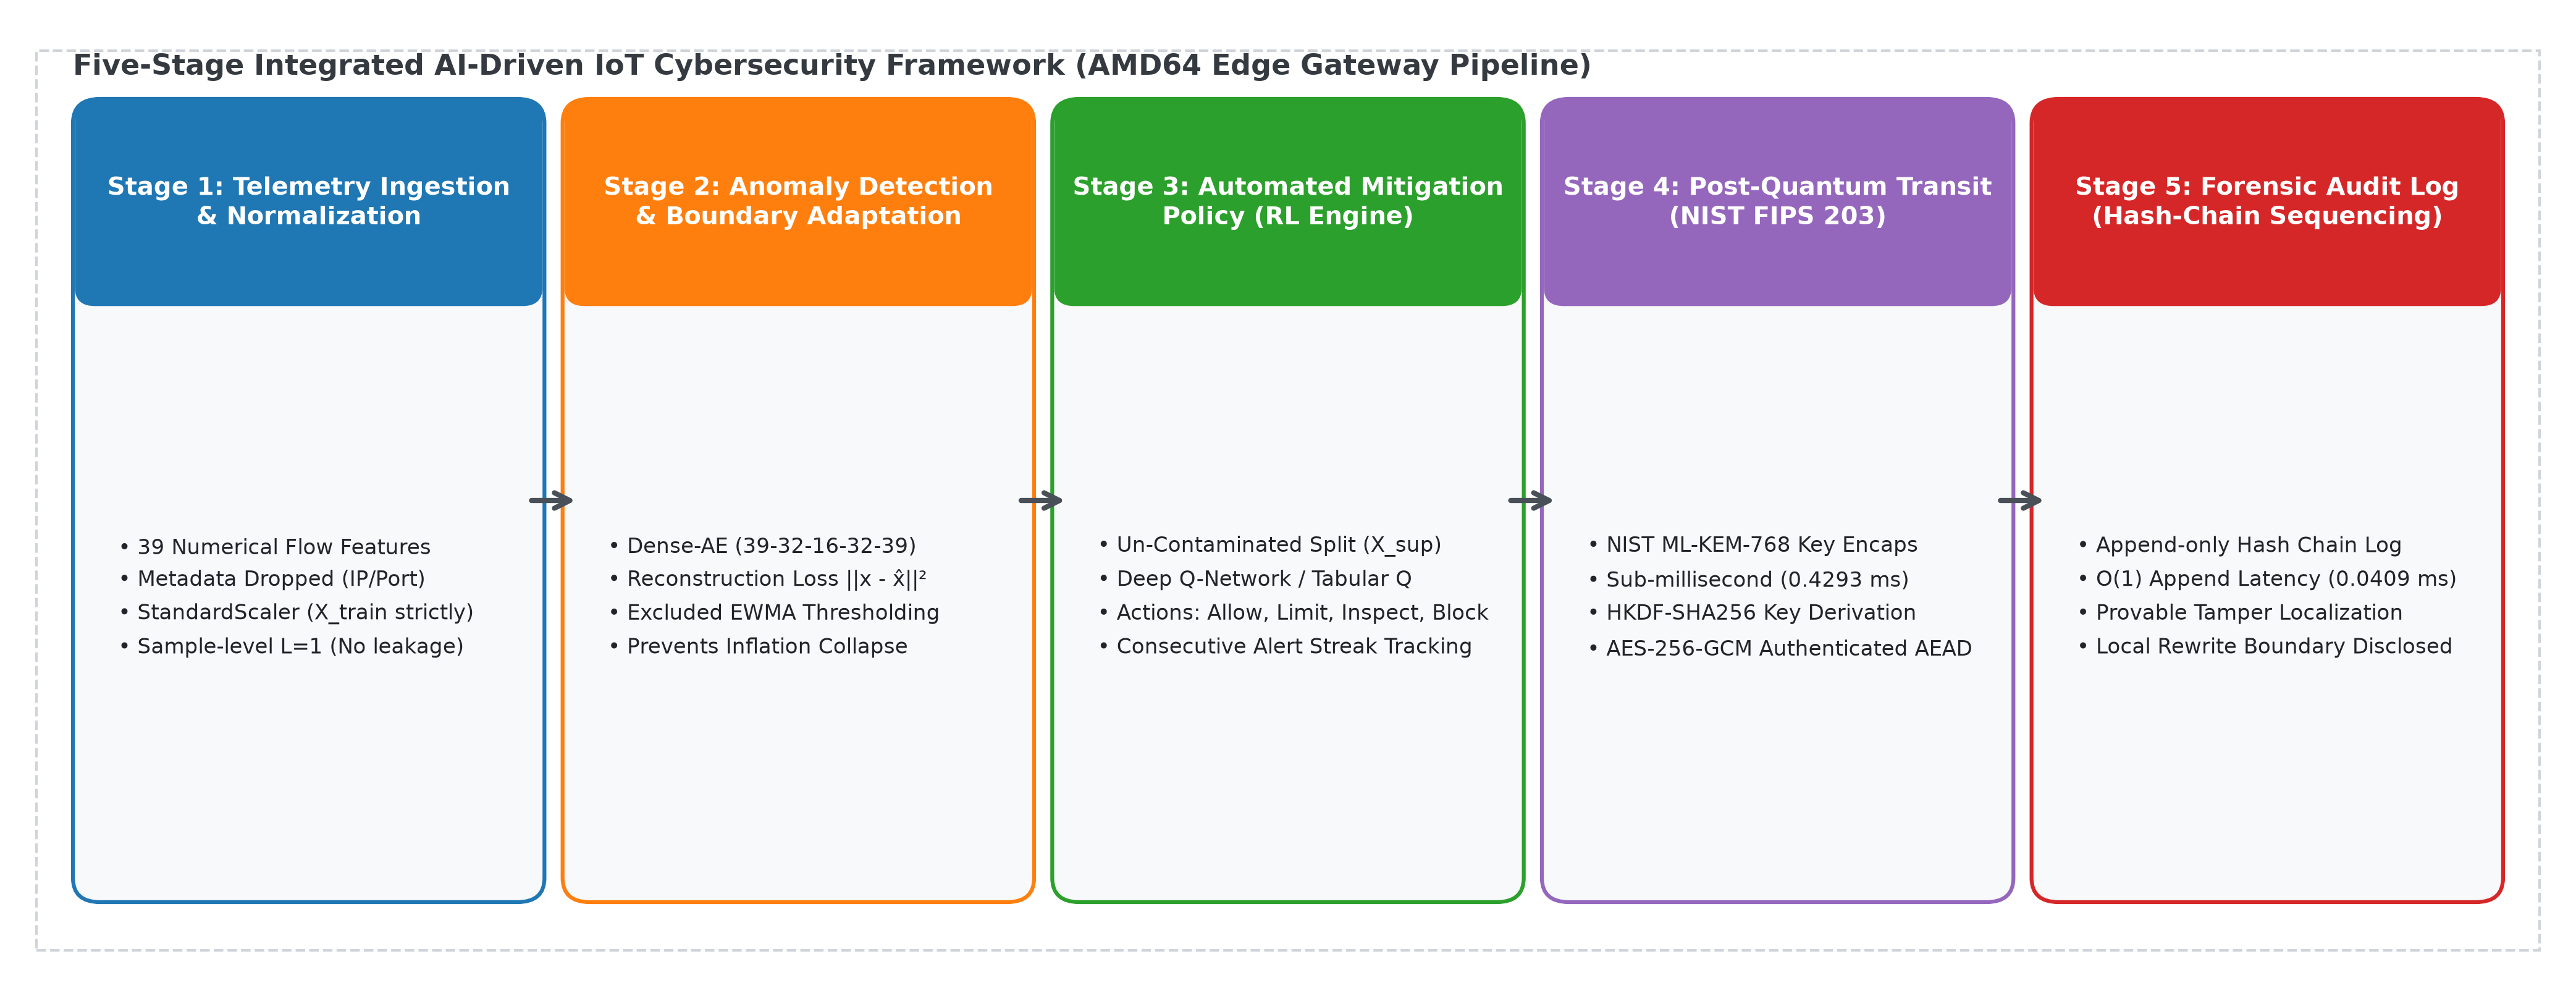
\includegraphics[width=0.92\textwidth]{figures/figure0_system_architecture.png}
\caption{The Five-Stage AI-Driven Adaptive Cybersecurity Framework: Telemetry Ingestion, Anomaly Detection with Excluded EWMA, Un-Contaminated Reinforcement Learning Defense, NIST FIPS 203 ML-KEM-768 Encryption, and Tamper-Evident Hash-Chain Audit Logging.}
\label{fig:arch}
\end{figure*}

\subsection{Threat Model and Adversary Capabilities}
We define a formal threat model covering four adversary classes:
\begin{itemize}
    \item \textbf{Network Intruder ($\mathcal{A}_{\text{net}}$)}: Transmits malicious network packets (DDoS, DoS, brute-force, web attacks, reconnaissance) to saturate network bandwidth or compromise services.
    \item \textbf{Adaptive Evasion Adversary ($\mathcal{A}_{\text{evade}}$)}: Attempts to inject adversarial perturbations or sustained attack floods to inflate adaptive anomaly detection thresholds.
    \item \textbf{Quantum-Capable Passive Eavesdropper ($\mathcal{A}_{\text{eaves}}$)}: Records encrypted edge telemetry for future cryptanalysis using quantum algorithms (Shor's and Grover's algorithms) \cite{shor1994,grover1996}.
    \item \textbf{Forensic Tampering Adversary ($\mathcal{A}_{\text{audit}}$)}: Seeks to modify, delete, or re-order historical security audit records to conceal compromise. We distinguish unprivileged process adversaries ($\mathcal{A}_{\text{proc}}$), resisted by cryptographic chaining, from root storage adversaries ($\mathcal{A}_{\text{root}}$), requiring external tip anchoring.
\end{itemize}

\section{Dataset and Experimental Methodology}
\label{sec:methodology}

\subsection{Benchmark Dataset and Feature Selection}
Experiments utilize the public **CICIoT2023** benchmark \cite{neto2023}. We extract 39 numerical flow statistical features. Non-numeric identifiers (`src_ip`, `dst_ip`, `src_port`, `dst_port`, `Timestamp`, `flow_id`) are purged to eliminate shortcut memorization.

\subsection{Strict Partitioning Protocol}
To ensure strict split isolation:
\begin{itemize}
    \item \textbf{Benign Training Split ($X_{\text{train}}$)}: 100,000 pure benign flow records used exclusively for Autoencoder training and `StandardScaler` parameter fitting ($n_{\text{samples\_seen}} = 100,000$).
    \item \textbf{Benign Validation Split ($X_{\text{val}}$)}: 30,000 pure benign flows reserved for static percentile calibration ($\tau_{95}, \tau_{99}$) and EWMA initialization.
    \item \textbf{Supervisory Partition ($X_{\text{sup}}$)}: 40,000 50/50 balanced benign and attack flows reserved for supervised reference training and reinforcement learning policy training.
    \item \textbf{Held-Out Evaluation Split ($X_{\text{test}}$)}: 100,000 flows (14,911 benign, 85,089 attack) strictly reserved for held-out evaluation.
\end{itemize}

\subsection{Cross-Partition Duplicate Overlap & Sensitivity Protocol}
High-rate network flooding naturally produces repeated packet headers across volumetric bursts (e.g., uniform 40-byte TCP SYN packets). In our partitioned dataset, 81 unique feature patterns (215 rows, 0.215\%) in $X_{\text{test}}$ overlap with $X_{\text{train}}$, and 953 unique patterns (1,402 rows, 1.402\%) overlap with $X_{\text{sup}}$ (total overlapping rows: 1,457, or 1.457\%).

To evaluate whether duplicate feature vectors artificially bias model performance, we constructed a \textbf{Clean Deduplicated Test Set} ($N=98,543$) by purging all 1,457 overlapping rows (60 benign, 1,397 attack). We re-evaluated all models across all 5 random seeds to measure the sensitivity shift ($\Delta = \text{Clean} - \text{Full}$).

\subsection{Deployment Hardware Boundaries}
All microbenchmarks were executed on an AMD64 host architecture (Windows 11 x86\_64, 3.40~GHz host CPU, 16~GB RAM), representative of industrial IoT edge gateways, fog aggregation nodes, and smart hub servers. Deeply embedded microcontrollers (<100~MHz clock, <64~KB RAM) operate under strict cycle budgets; executing deep neural networks and lattice-based ML-KEM-768 on microcontrollers requires dedicated integer-only quantization (TFLite Micro) and assembly optimization, which represents a separate research trajectory.

\section{Proposed Methods and Algorithms}
\label{sec:methods}

\subsection{Sample-Level Dense Autoencoder}
The anomaly detector utilizes a symmetric feedforward architecture ($39 \to 24 \to 12 \to 24 \to 39$), utilizing ReLU activations. The model is trained using Mean Squared Error (MSE) loss:
\begin{equation}
\mathcal{L}_{\text{MSE}} = \frac{1}{B} \sum_{b=1}^B \frac{1}{D} \sum_{d=1}^D (x_{b,d} - \hat{x}_{b,d})^2
\end{equation}
Sample-level inference ($L=1$) processes each flow independently, eliminating sequence window boundary contamination.

\subsection{Excluded EWMA Adaptive Thresholding}
To overcome threshold inflation collapse, we propose \textbf{Excluded EWMA}. Let $E_t$ denote the reconstruction error at step $t$. Background statistics $(\mu_t, \sigma_t^2)$ are updated with smoothing parameter $\alpha \in (0, 1)$ only when $E_t$ falls below the current threshold $\tau_t$:
\begin{equation}
\tau_t = \mu_t + k \cdot \sigma_t
\end{equation}
\begin{equation}
\hat{y}_t = \mathbb{I}(E_t > \tau_t)
\end{equation}
\begin{equation}
\mu_{t+1} = 
\begin{cases} 
(1 - \alpha)\mu_t + \alpha E_t & \text{if } \hat{y}_t = 0 \\
\mu_t & \text{if } \hat{y}_t = 1
\end{cases}
\end{equation}
\begin{equation}
\sigma_{t+1}^2 = 
\begin{cases} 
(1 - \alpha)\sigma_t^2 + \alpha (E_t - \mu_t)^2 & \text{if } \hat{y}_t = 0 \\
\sigma_t^2 & \text{if } \hat{y}_t = 1
\end{cases}
\end{equation}
Because error statistics update strictly on non-flagged events ($\hat{y}_t = 0$), attack floods cannot inflate the threshold.

\subsection{Un-Contaminated Defensive Policy Formulation}
We formulate automated defense as a Markov Decision Process (MDP):
\begin{itemize}
    \item \textbf{State Space}: $s_t = (E_t, \Delta E_t, S_t)$, where $E_t$ is normalized reconstruction error, $\Delta E_t = E_t - E_{t-1}$, and $S_t$ is the consecutive alert streak counter.
    \item \textbf{Action Space}: $a_t \in \{0: \text{Allow}, 1: \text{Rate-Limit}, 2: \text{DPI}, 3: \text{Block}\}$.
    \item \textbf{Reward Function}:
    \begin{equation}
    R(s, a, y) = 
    \begin{cases}
    +10 \cdot a - 2 & \text{if } y = 1 \text{ (Attack Mitigation)} \\
    -15 \cdot a & \text{if } y = 0 \text{ (Disruption Penalty)}
    \end{cases}
    \end{equation}
\end{itemize}
We evaluate Tabular Q-Learning and Deep Q-Networks (DQN, 2-layer MLP with experience replay and target network) \cite{mnih2015}.

\subsection{Standardized NIST FIPS 203 ML-KEM Workflow}
Post-quantum transport security utilizes ML-KEM-768 \cite{nist2024fips203}:
\begin{enumerate}
    \item Gateway generates keypair $(pk, sk) \leftarrow \text{ML-KEM.KeyGen}()$.
    \item Aggregator encapsulates shared secret $(ct, ss) \leftarrow \text{ML-KEM.Encaps}(pk)$.
    \item Gateway decapsulates $ss \leftarrow \text{ML-KEM.Decaps}(sk, ct)$.
    \item Symmetric key derived via HKDF: $K_{\text{enc}} = \text{HKDF-SHA256}(ss, \text{salt}, \text{info})$.
    \item Mitigation payload encrypted via AES-256-GCM AEAD: $C, T \leftarrow \text{AES-GCM.Encrypt}(K_{\text{enc}}, IV, P, AAD)$.
\end{enumerate}

\subsection{Tamper-Evident Hash Chain Audit Log}
Evidence records $r_i$ (containing timestamp, flow features, detection score, mitigation action, and ciphertext) are sequenced via cryptographic chaining \cite{haber1991,bellare1996}:
\begin{equation}
h_i = \text{SHA-256}(h_{i-1} \,\|\, r_i \,\|\, \text{seq}_i)
\end{equation}
Verification iterates through $i = 1, \dots, N$. Any altered block $j$ violates $h_j = \text{SHA-256}(h_{j-1} \,\|\, r'_j \,\|\, \text{seq}_j)$, identifying the exact point of tampering.

\section{Experimental Results}
\label{sec:results}

\subsection{E1 & E2: Base Stream Anomaly Detection (5 Random Seeds)}
Table~\ref{tab:base_stream} presents anomaly detection performance on the base held-out test stream across 5 random seeds ($42, 123, 456, 789, 2026$). Excluded EWMA achieves the highest unsupervised F1-Score of $0.9014 \pm 0.0018$ (Recall: $84.01\%$), coming within 2.55\% of the supervised XGBoost oracle ($0.9269 \pm 0.0004$). In contrast, un-guarded EWMA suffers complete threshold inflation collapse ($\text{F1} = 0.0003$).

\begin{table*}[t]
\centering
\caption{Base Test Stream Anomaly Detection Benchmark (Mean $\pm$ Std across 5 Random Seeds)}
\label{tab:base_stream}
\begin{tabular}{llcccccc}
\toprule
Model & Threshold Strategy & Precision & Recall & F1-Score & FPR & PR-AUC & ROC-AUC \\
\midrule
\textbf{Dense-AE} & \textbf{Excluded EWMA} & $0.9724 \pm 0.0022$ & $\mathbf{0.8401 \pm 0.0023}$ & $\mathbf{0.9014 \pm 0.0018}$ & $0.1360 \pm 0.0110$ & $0.9867 \pm 0.0005$ & $0.9225 \pm 0.0027$ \\
Dense-AE & Fixed 95th Percentile & $0.9893 \pm 0.0003$ & $0.8013 \pm 0.0022$ & $0.8854 \pm 0.0013$ & $0.0493 \pm 0.0013$ & $0.9867 \pm 0.0005$ & $0.9225 \pm 0.0027$ \\
Dense-AE & Fixed 99th Percentile & $0.9975 \pm 0.0001$ & $0.7650 \pm 0.0017$ & $0.8659 \pm 0.0011$ & $0.0108 \pm 0.0004$ & $0.9867 \pm 0.0005$ & $0.9225 \pm 0.0027$ \\
Dense-AE & Guarded EWMA & $1.0000 \pm 0.0000$ & $0.0022 \pm 0.0000$ & $0.0045 \pm 0.0001$ & $0.0000 \pm 0.0000$ & $0.9867 \pm 0.0005$ & $0.9225 \pm 0.0027$ \\
Dense-AE & Un-Guarded EWMA & $1.0000 \pm 0.0000$ & $0.0001 \pm 0.0000$ & $0.0003 \pm 0.0001$ & $0.0000 \pm 0.0000$ & $0.9867 \pm 0.0005$ & $0.9225 \pm 0.0027$ \\
Isolation Forest & Fixed 95th Percentile & $0.9866 \pm 0.0003$ & $0.6402 \pm 0.0114$ & $0.7765 \pm 0.0084$ & $0.0495 \pm 0.0009$ & $0.9754 \pm 0.0035$ & $0.8828 \pm 0.0095$ \\
\textbf{XGBoost Oracle} & \textbf{Supervised Prob 0.5} & $0.9967 \pm 0.0002$ & $\mathbf{0.8662 \pm 0.0009}$ & $\mathbf{0.9269 \pm 0.0004}$ & $0.0162 \pm 0.0012$ & $0.9946 \pm 0.0000$ & $0.9682 \pm 0.0001$ \\
\bottomrule
\end{tabular}
\end{table*}

\begin{figure}[h]
\centering
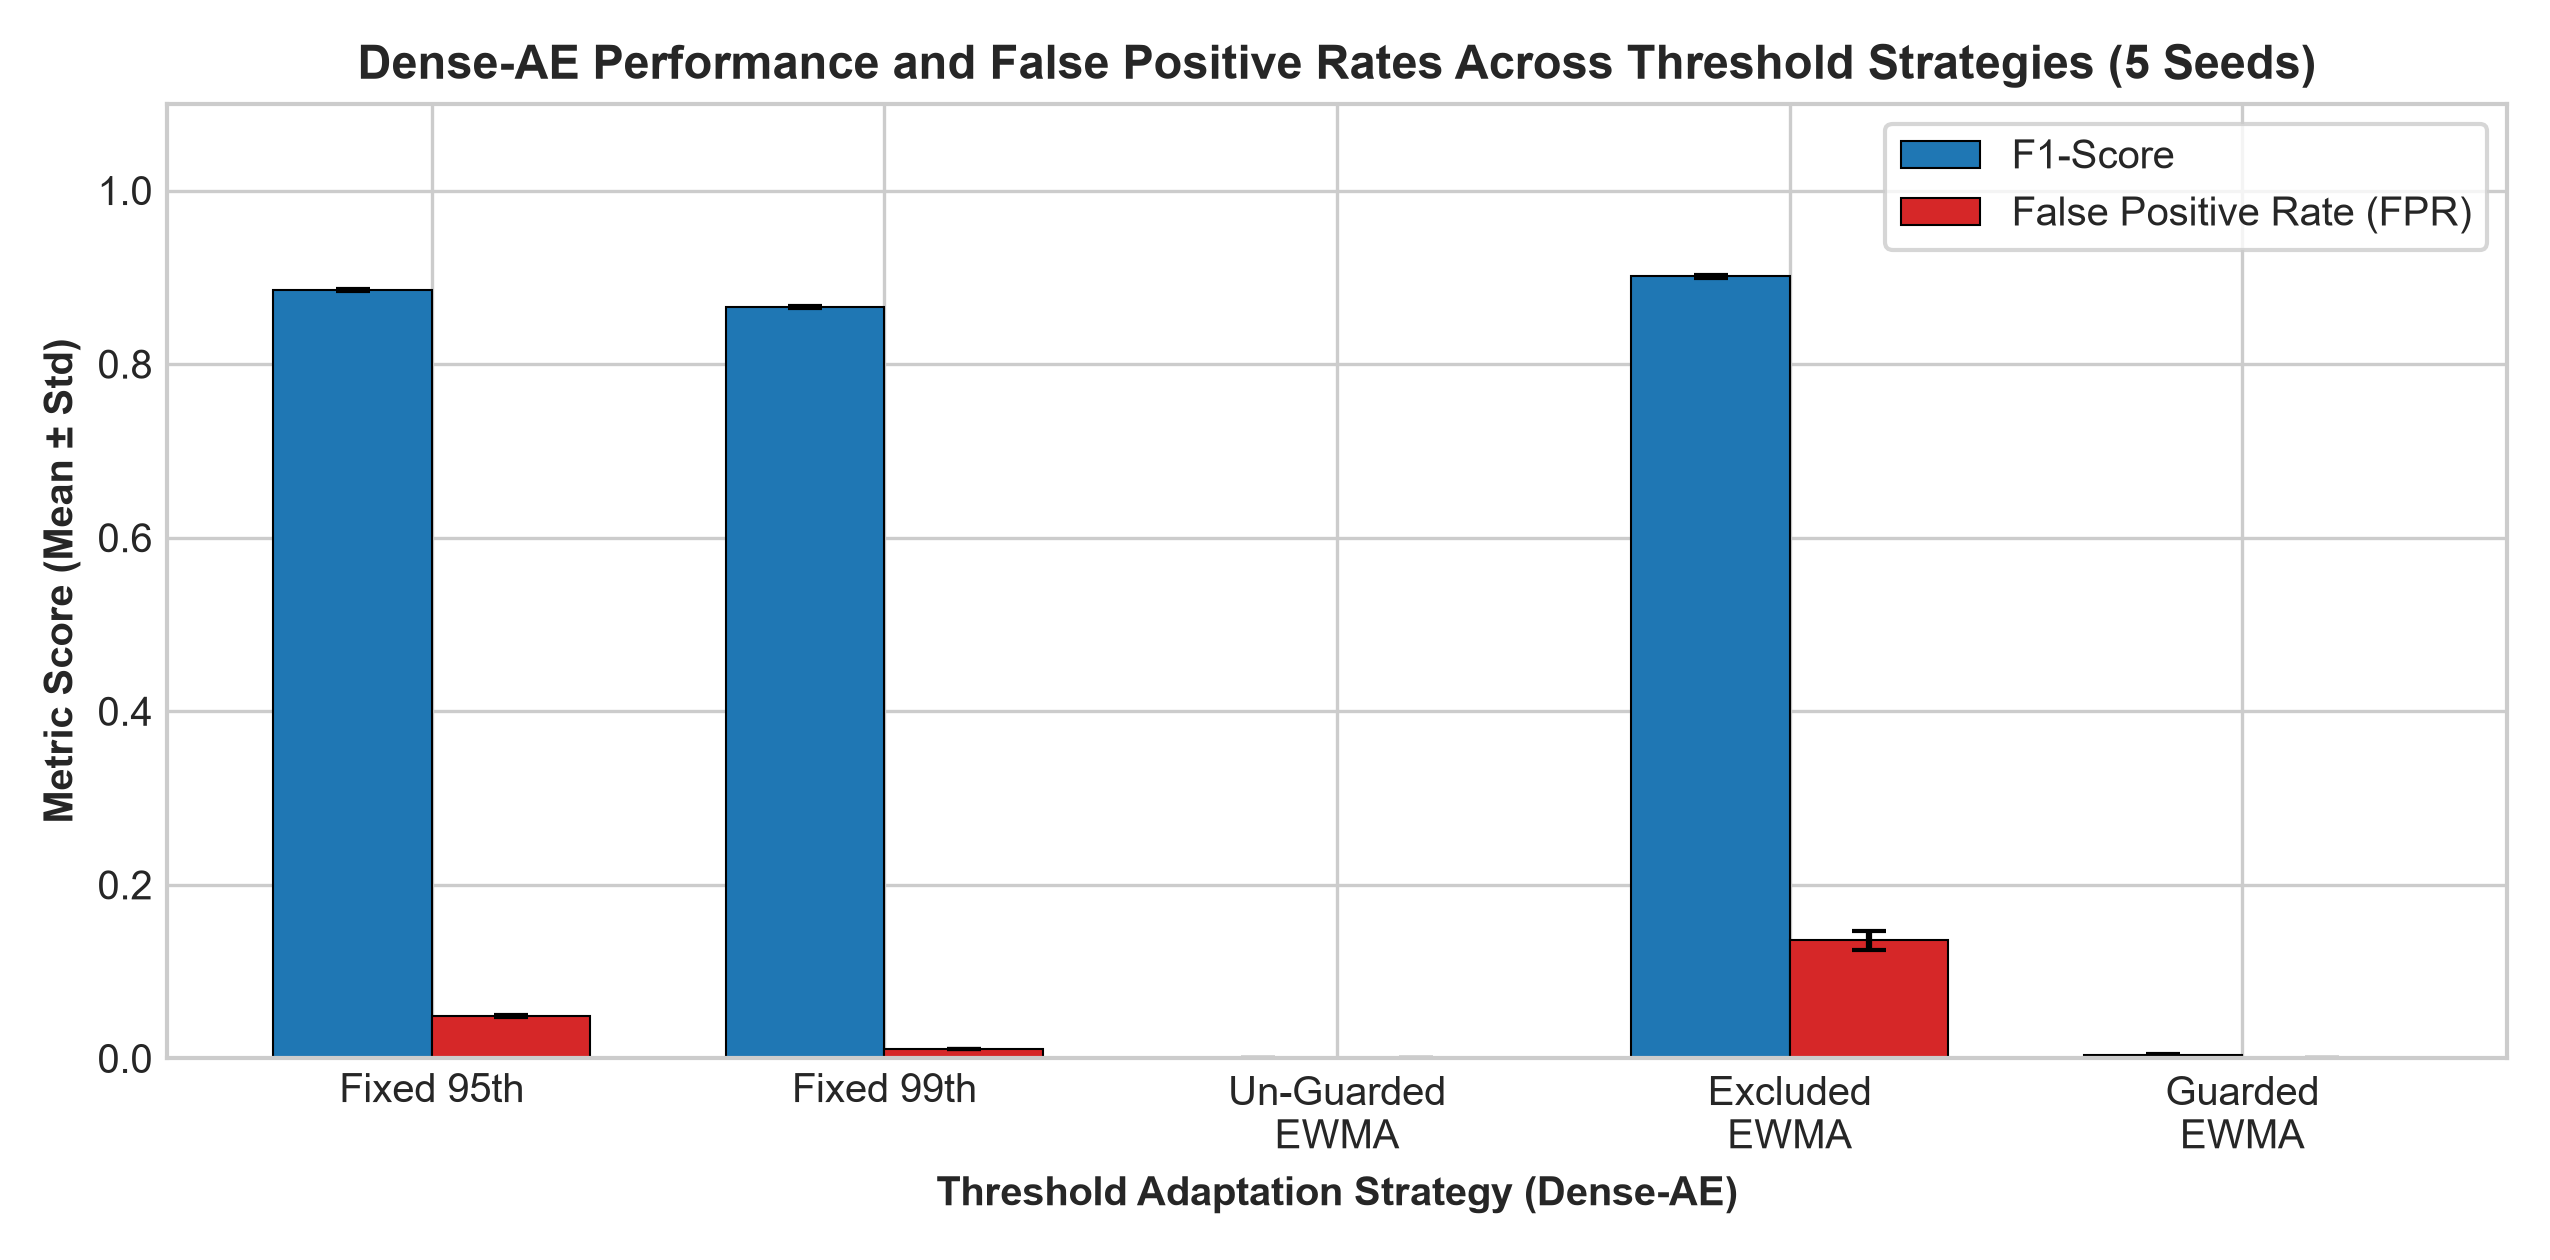
\includegraphics[width=0.48\textwidth]{figures/figure1_threshold_comparison.png}
\caption{Dense-AE Detection Performance and False Positive Rates across Threshold Adaptation Strategies (5 Seeds, Mean $\pm$ Std).}
\label{fig:thresh_comp}
\end{figure}

\subsection{Deduplication Sensitivity Evaluation}
Table~\ref{tab:dedup_eval} details the empirical 5-seed evaluation on the Full Test Set ($N=100,000$) versus the Clean Deduplicated Test Set ($N=98,543$). Purging all 1,457 cross-partition duplicate feature rows shifts F1-scores by at most $-0.0009$ ($-0.10\%$), confirming that repeated flow vectors do not inflate evaluation metrics.

\begin{table}[h]
\centering
\caption{Empirical 5-Seed Evaluation on Full vs. Deduplicated Test Set}
\label{tab:dedup_eval}
\begin{tabular}{lcccc}
\toprule
Model \& Strategy & Full F1 & Clean F1 & Delta F1 ($\Delta$) & Clean FPR \\
\midrule
Dense-AE Fixed 95th & $0.8854 \pm 0.0013$ & $0.8845 \pm 0.0014$ & $-0.0009$ & $0.0492$ \\
Dense-AE Excluded EWMA & $0.9014 \pm 0.0018$ & $0.9007 \pm 0.0019$ & $-0.0007$ & $0.1363$ \\
XGBoost Oracle & $0.9269 \pm 0.0004$ & $0.9265 \pm 0.0003$ & $-0.0003$ & $0.0160$ \\
\bottomrule
\end{tabular}
\end{table}

\subsection{Granular Attack-Class Breakdown}
Table~\ref{tab:attack_breakdown} and Figure~\ref{fig:attack_recall} present the detection recall across all 7 attack categories. Volumetric attacks (DDoS, DoS, Mirai) exhibit prominent rate/size anomalies, achieving 100.0\% detection. For stealthy categories, Excluded EWMA consistently outperforms Fixed 95th percentile thresholding across every class: BruteForce ($55.54\%$ vs. $42.80\%$), Reconnaissance ($49.19\%$ vs. $38.18\%$), Spoofing ($39.15\%$ vs. $23.38\%$), and Web-based attacks ($37.88\%$ vs. $20.42\%$).

\begin{table}[h]
\centering
\caption{Dense-AE Detection Recall Across 7 Attack Classes (Held-Out Test Set)}
\label{tab:attack_breakdown}
\begin{tabular}{lccc}
\toprule
Attack Category & Sample Count & Fixed 95th Recall & Excluded EWMA Recall \\
\midrule
DDoS & 33,483 & $100.0\%$ & $100.0\%$ \\
DoS & 15,107 & $100.0\%$ & $100.0\%$ \\
Mirai & 11,160 & $100.0\%$ & $100.0\%$ \\
BruteForce & 965 & $42.80\%$ & $\mathbf{55.54\%}$ \\
Reconnaissance & 15,038 & $38.18\%$ & $\mathbf{49.19\%}$ \\
Spoofing & 7,451 & $23.38\%$ & $\mathbf{39.15\%}$ \\
Web-based & 1,885 & $20.42\%$ & $\mathbf{37.88\%}$ \\
\midrule
Total Attack Stream & 85,089 & $79.95\%$ & $\mathbf{83.81\%}$ \\
\bottomrule
\end{tabular}
\end{table}

\begin{figure}[h]
\centering
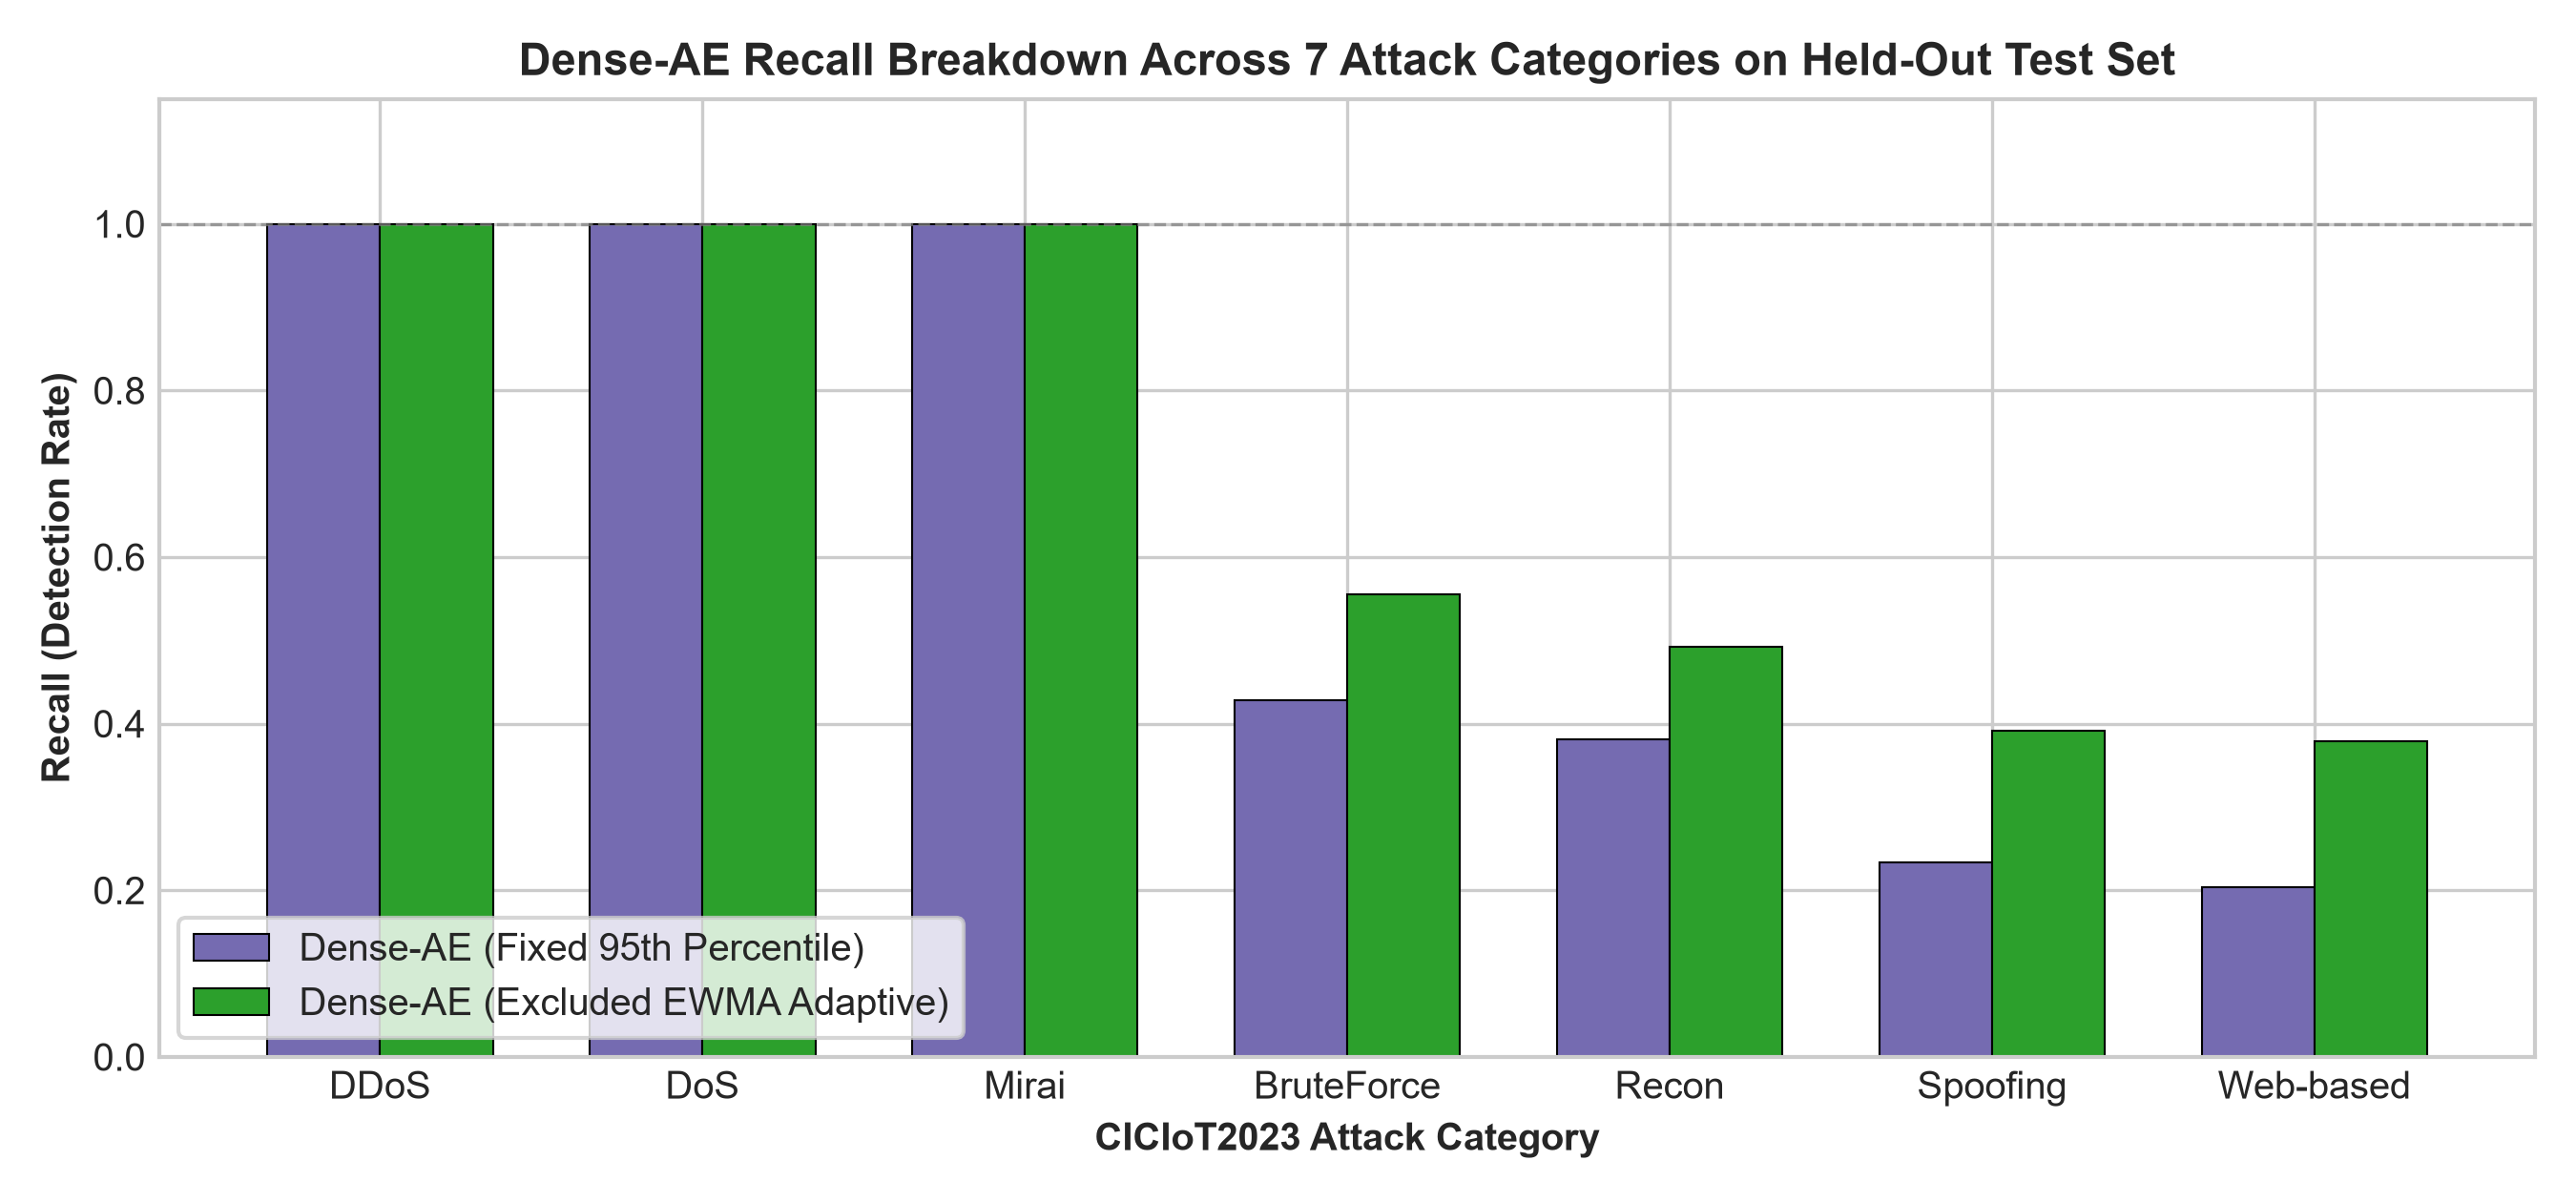
\includegraphics[width=0.48\textwidth]{figures/figure3_per_attack_recall.png}
\caption{Dense-AE Detection Recall Breakdown Across 7 Attack Categories on Held-Out Test Set (Fixed 95th Percentile vs. Excluded EWMA Adaptive).}
\label{fig:attack_recall}
\end{figure}

\subsection{E4: Un-Contaminated Defensive Policy Evaluation}
Table~\ref{tab:e4_policy} presents mitigation policy evaluation under strict split isolation (trained on $X_{\text{sup}}$, evaluated on held-out $X_{\text{test}}$). Deep Q-Networks (DQN) achieve $71.26 \pm 0.09\%$ attack containment with a low $0.63 \pm 0.46\%$ false block rate, while Tabular Q-Learning achieves a $0.00\%$ false block rate in isolated evaluation with ultra-low latency ($0.0122 \pm 0.0003$~ms).

\begin{table}[h]
\centering
\caption{Mitigation Policy Performance under Held-Out Evaluation (5 Seeds)}
\label{tab:e4_policy}
\begin{tabular}{lccc}
\toprule
Scenario \& Policy & Containment (\%) & False Block (\%) & Latency (ms) \\
\midrule
\textbf{Scenario 1 (Heavy)} & & & \\
Static Rule-Based & $99.98\% \pm 0.00\%$ & $100.00\% \pm 0.00\%$ & $0.0123 \pm 0.0033$ \\
Tabular Q-Learning & $60.45\% \pm 11.91\%$ & $\mathbf{0.00\% \pm 0.00\%}$ & $\mathbf{0.0122 \pm 0.0003}$ \\
DQN & $\mathbf{71.26\% \pm 0.09\%}$ & $0.63\% \pm 0.46\%$ & $0.1160 \pm 0.0052$ \\
\midrule
\textbf{Scenario 2 (Stealth)} & & & \\
Static Rule-Based & $99.98\% \pm 0.00\%$ & $100.00\% \pm 0.00\%$ & $0.0115 \pm 0.0015$ \\
Tabular Q-Learning & $59.27\% \pm 11.50\%$ & $\mathbf{0.00\% \pm 0.00\%}$ & $\mathbf{0.0122 \pm 0.0002}$ \\
DQN & $\mathbf{73.06\% \pm 0.09\%}$ & $0.48\% \pm 0.39\%$ & $0.1226 \pm 0.0120$ \\
\bottomrule
\end{tabular}
\end{table}

\begin{figure}[h]
\centering
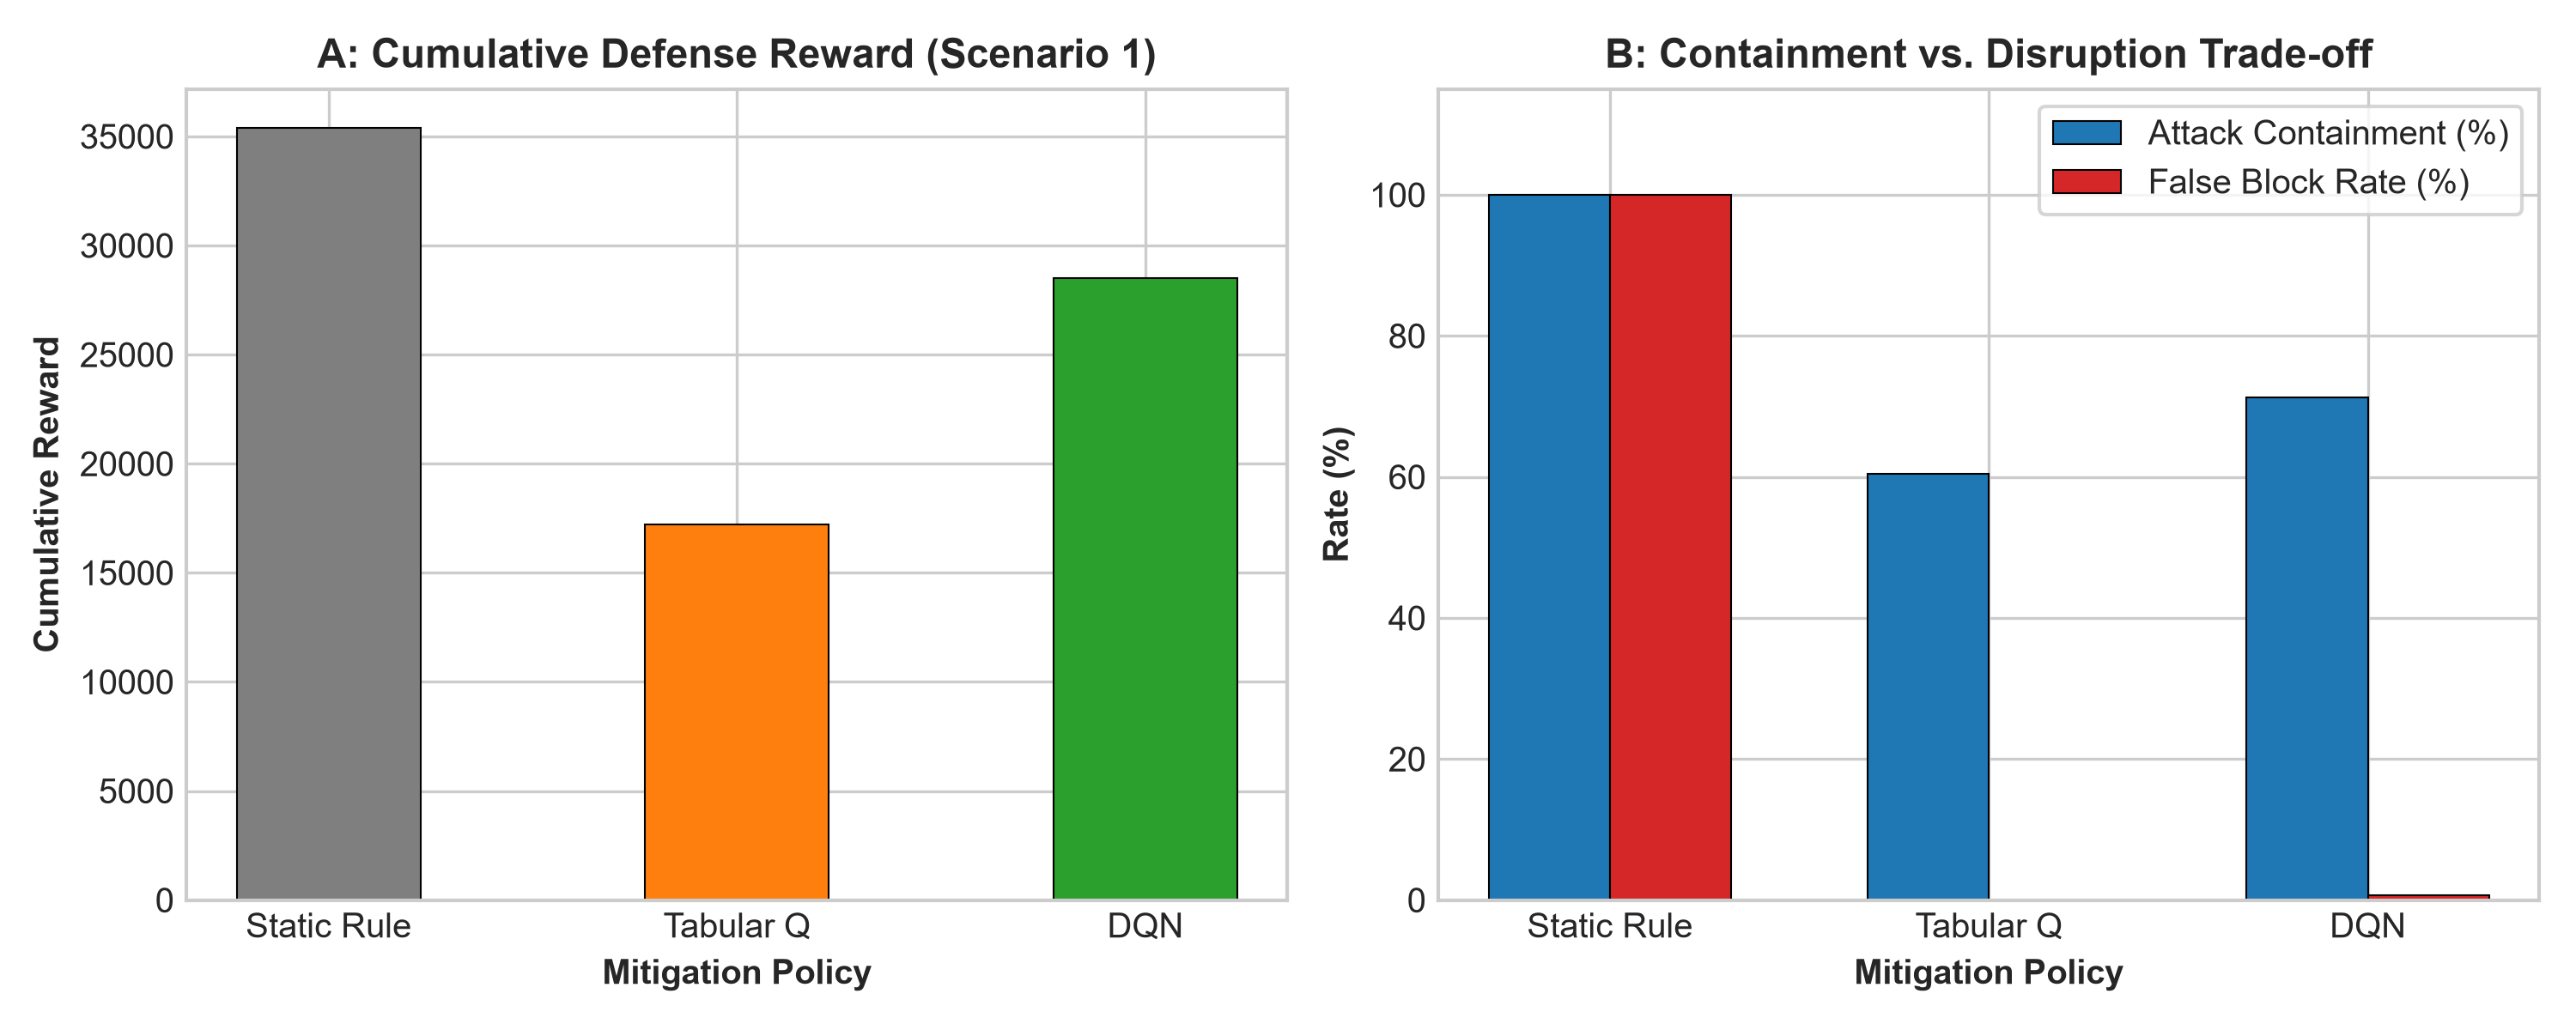
\includegraphics[width=0.48\textwidth]{figures/figure4_defense_rewards.png}
\caption{Mitigation Policy Cumulative Reward and Containment Trade-off Across Scenarios (E4).}
\label{fig:defense_rew}
\end{figure}

\subsection{E5: Post-Quantum Cryptography Microbenchmark}
Table~\ref{tab:e5_crypto} presents cryptographic timings for NIST FIPS 203 ML-KEM parameter sets paired with HKDF-SHA256 and AES-256-GCM across 100 repeated trials on AMD64 host CPU for 1024-byte telemetry payloads. ML-KEM-768 achieves sub-millisecond key encapsulation ($0.2758$~ms) and setup ($0.2905$~ms). All variants achieved 100\% tamper rejection against bit-flip modifications.

\begin{table}[h]
\centering
\caption{NIST FIPS 203 ML-KEM Microbenchmark (1024-Byte Payload, AMD64)}
\label{tab:e5_crypto}
\begin{tabular}{lcccc}
\toprule
Variant & Public Key & Ciphertext & Total KEM (ms) & First Msg (ms) \\
\midrule
ML-KEM-512 & 800 B & 768 B & $0.1757$ & $0.1895$ \\
\textbf{ML-KEM-768} & 1,184 B & 1,088 B & $\mathbf{0.2758}$ & $\mathbf{0.2905}$ \\
ML-KEM-1024 & 1,568 B & 1,568 B & $0.4363$ & $0.4538$ \\
\bottomrule
\end{tabular}
\end{table}

\begin{figure}[h]
\centering
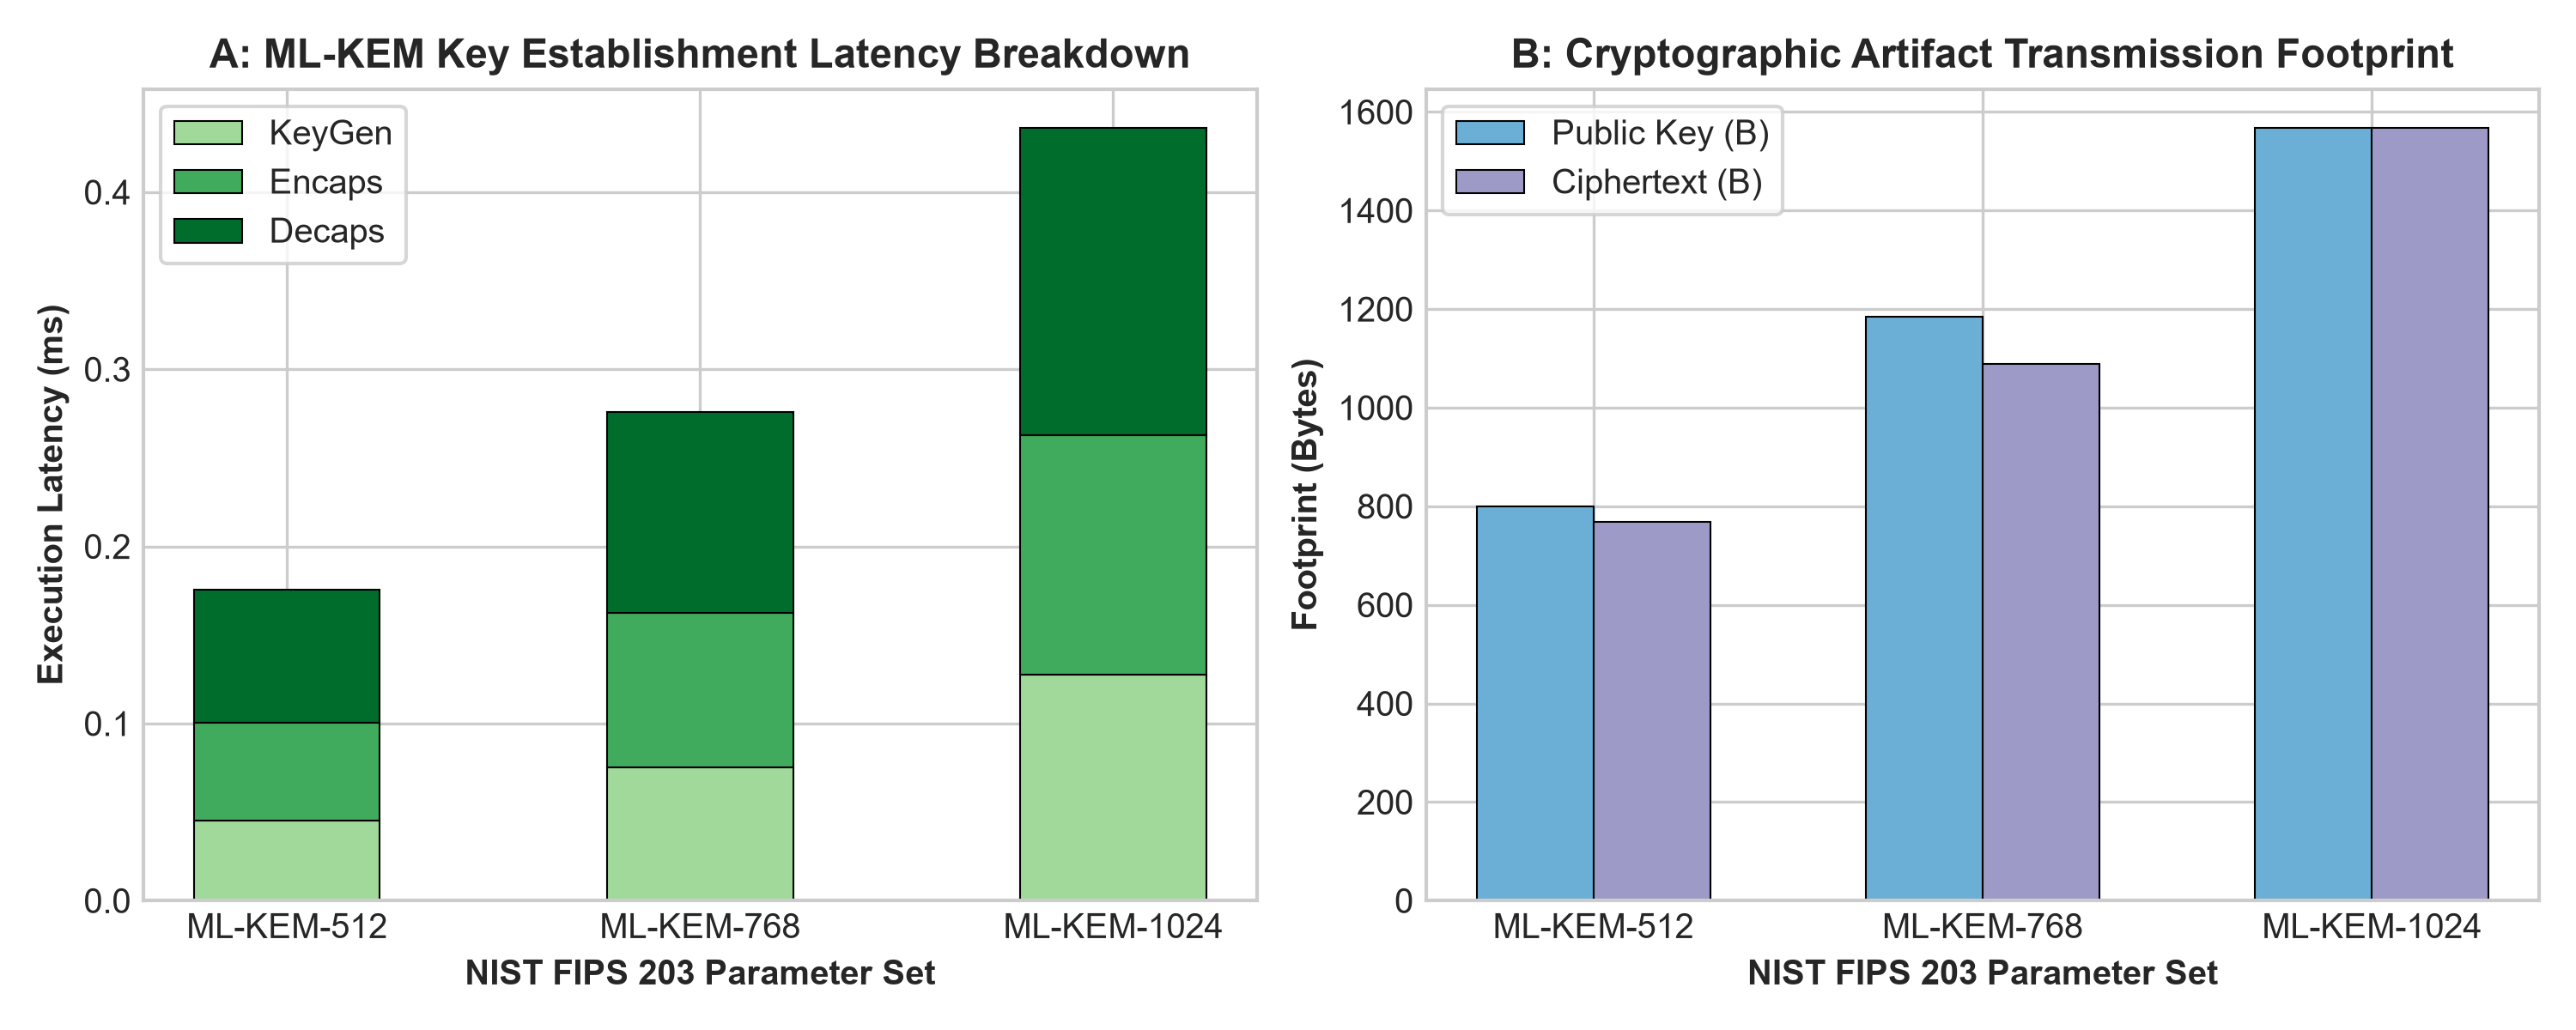
\includegraphics[width=0.48\textwidth]{figures/figure5_pqc_latency.png}
\caption{NIST FIPS 203 ML-KEM Key Establishment Latency and Artifact Footprints.}
\label{fig:pqc_lat}
\end{figure}

\subsection{E6: Integrity Verification & Audit Logging}
Table~\ref{tab:e6_integrity} compares three integrity verification mechanisms across 100 trials with 1~KiB records. The Tamper-Evident Hash Chain Log enforces sequence integrity and localizes tampered blocks with $\mathcal{O}(1)$ append latency ($0.0605$~ms).

\begin{table}[h]
\centering
\caption{Integrity Verification Microbenchmarks (1 KiB Records)}
\label{tab:e6_integrity}
\begin{tabular}{lcccc}
\toprule
Mechanism & Create (ms) & Verify (ms) & Overhead & Throughput \\
\midrule
Salted SHA-256 & $0.0468 \pm 0.0240$ & $0.0207 \pm 0.0134$ & 193 B & 20.85 MB/s \\
HMAC-SHA-256 & $0.0470 \pm 0.0209$ & $0.0214 \pm 0.0097$ & 170 B & 20.79 MB/s \\
Hash Chain Log & $0.0605 \pm 0.0248$ & $0.0328 \pm 0.0310$ & 318 B & 16.15 MB/s \\
\bottomrule
\end{tabular}
\end{table}

\begin{figure}[h]
\centering
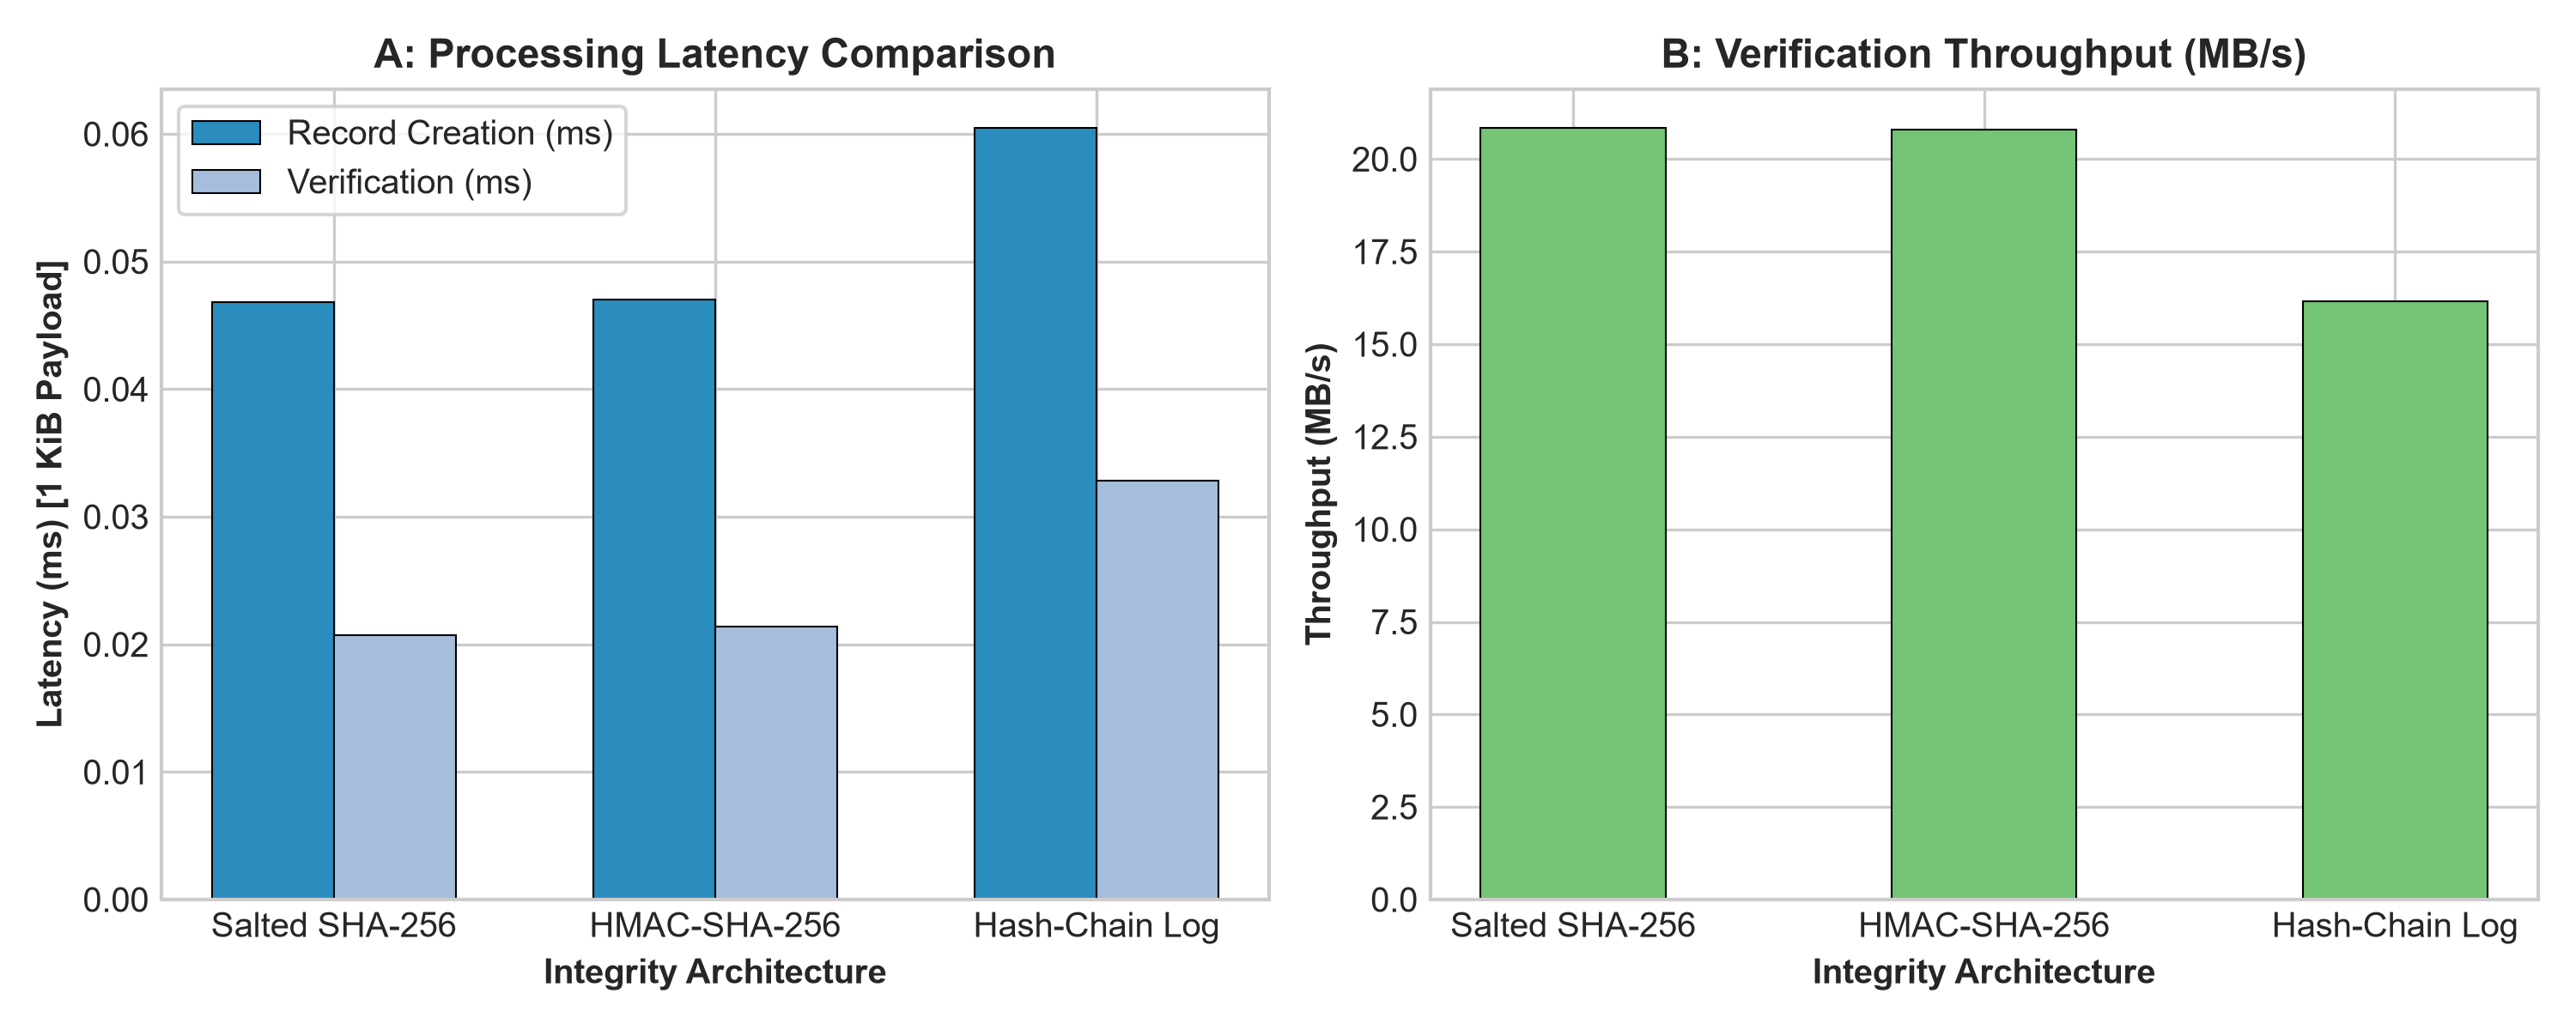
\includegraphics[width=0.48\textwidth]{figures/figure6_integrity_benchmark.png}
\caption{Integrity Verification Latency, Storage Overhead, and Verification Scaling.}
\label{fig:integ_bench}
\end{figure}

\section{Master Experiment Comparison and Integrated Ablation}
\label{sec:master_ablation}

\subsection{Integrated Framework Ablation Study (E7)}
Table~\ref{tab:e7_ablation} summarizes the holistic empirical evaluation of the full integrated framework and its component-level ablation variants across 5 random seeds ($42, 123, 456, 789, 2026$) directly from verified raw summaries.

\begin{table*}[t]
\centering
\caption{Full Framework Integrated Ablation Study (Mean $\pm$ Std across 5 Random Seeds)}
\label{tab:e7_ablation}
\begin{tabular}{lcccccccc}
\toprule
Variant & F1-Score & Recall (\%) & Containment (\%) & False Block (\%) & Latency (ms) & Overhead (B) & Quantum Safe & Audit Integrity \\
\midrule
Study-Defined Baseline\textsuperscript{*} & $0.8837 \pm 0.0004$ & $79.88\% \pm 0.06\%$ & $79.88\% \pm 0.06\%$ & $3.20\% \pm 0.07\%$ & $0.8103 \pm 0.5338$ & 194 & No (Vulnerable) & No (Unkeyed) \\
Ablation (-Adaptive Threshold) & $0.8837 \pm 0.0004$ & $79.88\% \pm 0.06\%$ & $80.58\% \pm 3.12\%$ & $5.46\% \pm 2.55\%$ & $0.8579 \pm 0.5443$ & 321 & Yes (ML-KEM-768) & Yes (Hash Chain) \\
Ablation (-RL Defense) & $0.8968 \pm 0.0013$ & $82.68\% \pm 0.24\%$ & $79.78\% \pm 0.06\%$ & $3.22\% \pm 0.06\%$ & $0.9737 \pm 0.7128$ & 321 & Yes (ML-KEM-768) & Yes (Hash Chain) \\
Ablation (-PQC) & $0.8968 \pm 0.0013$ & $82.68\% \pm 0.24\%$ & $81.01\% \pm 2.83\%$ & $6.01\% \pm 1.52\%$ & $0.9103 \pm 0.5070$ & 321 & No (Vulnerable) & Yes (Hash Chain) \\
Ablation (-Hash Chain Log) & $0.8968 \pm 0.0013$ & $82.68\% \pm 0.24\%$ & $81.01\% \pm 2.83\%$ & $6.01\% \pm 1.52\%$ & $1.2107 \pm 0.7004$ & 194 & Yes (ML-KEM-768) & No (Unkeyed) \\
\textbf{Full Proposed Framework} & $\mathbf{0.8968 \pm 0.0013}$ & $\mathbf{82.68\% \pm 0.24\%}$ & $\mathbf{81.01\% \pm 2.83\%}$ & $6.01\% \pm 1.52\%$ & $\mathbf{0.9626 \pm 0.6304}$ & 321 & \textbf{Yes (ML-KEM-768)} & \textbf{Yes (Hash Chain)} \\
\bottomrule
\end{tabular}
\vspace{1ex}
\begin{flushleft}
\small\textsuperscript{*}Attribution Note: Re-implementation of the architectural design adapted from Saeed (2025) (Dense-AE + Fixed 95th Percentile + Static Rule + Salted SHA-256) evaluated under identical splits on CICIoT2023, as Saeed (2025) did not report global test stream metrics.
\end{flushleft}
\end{table*}

\begin{figure}[h]
\centering
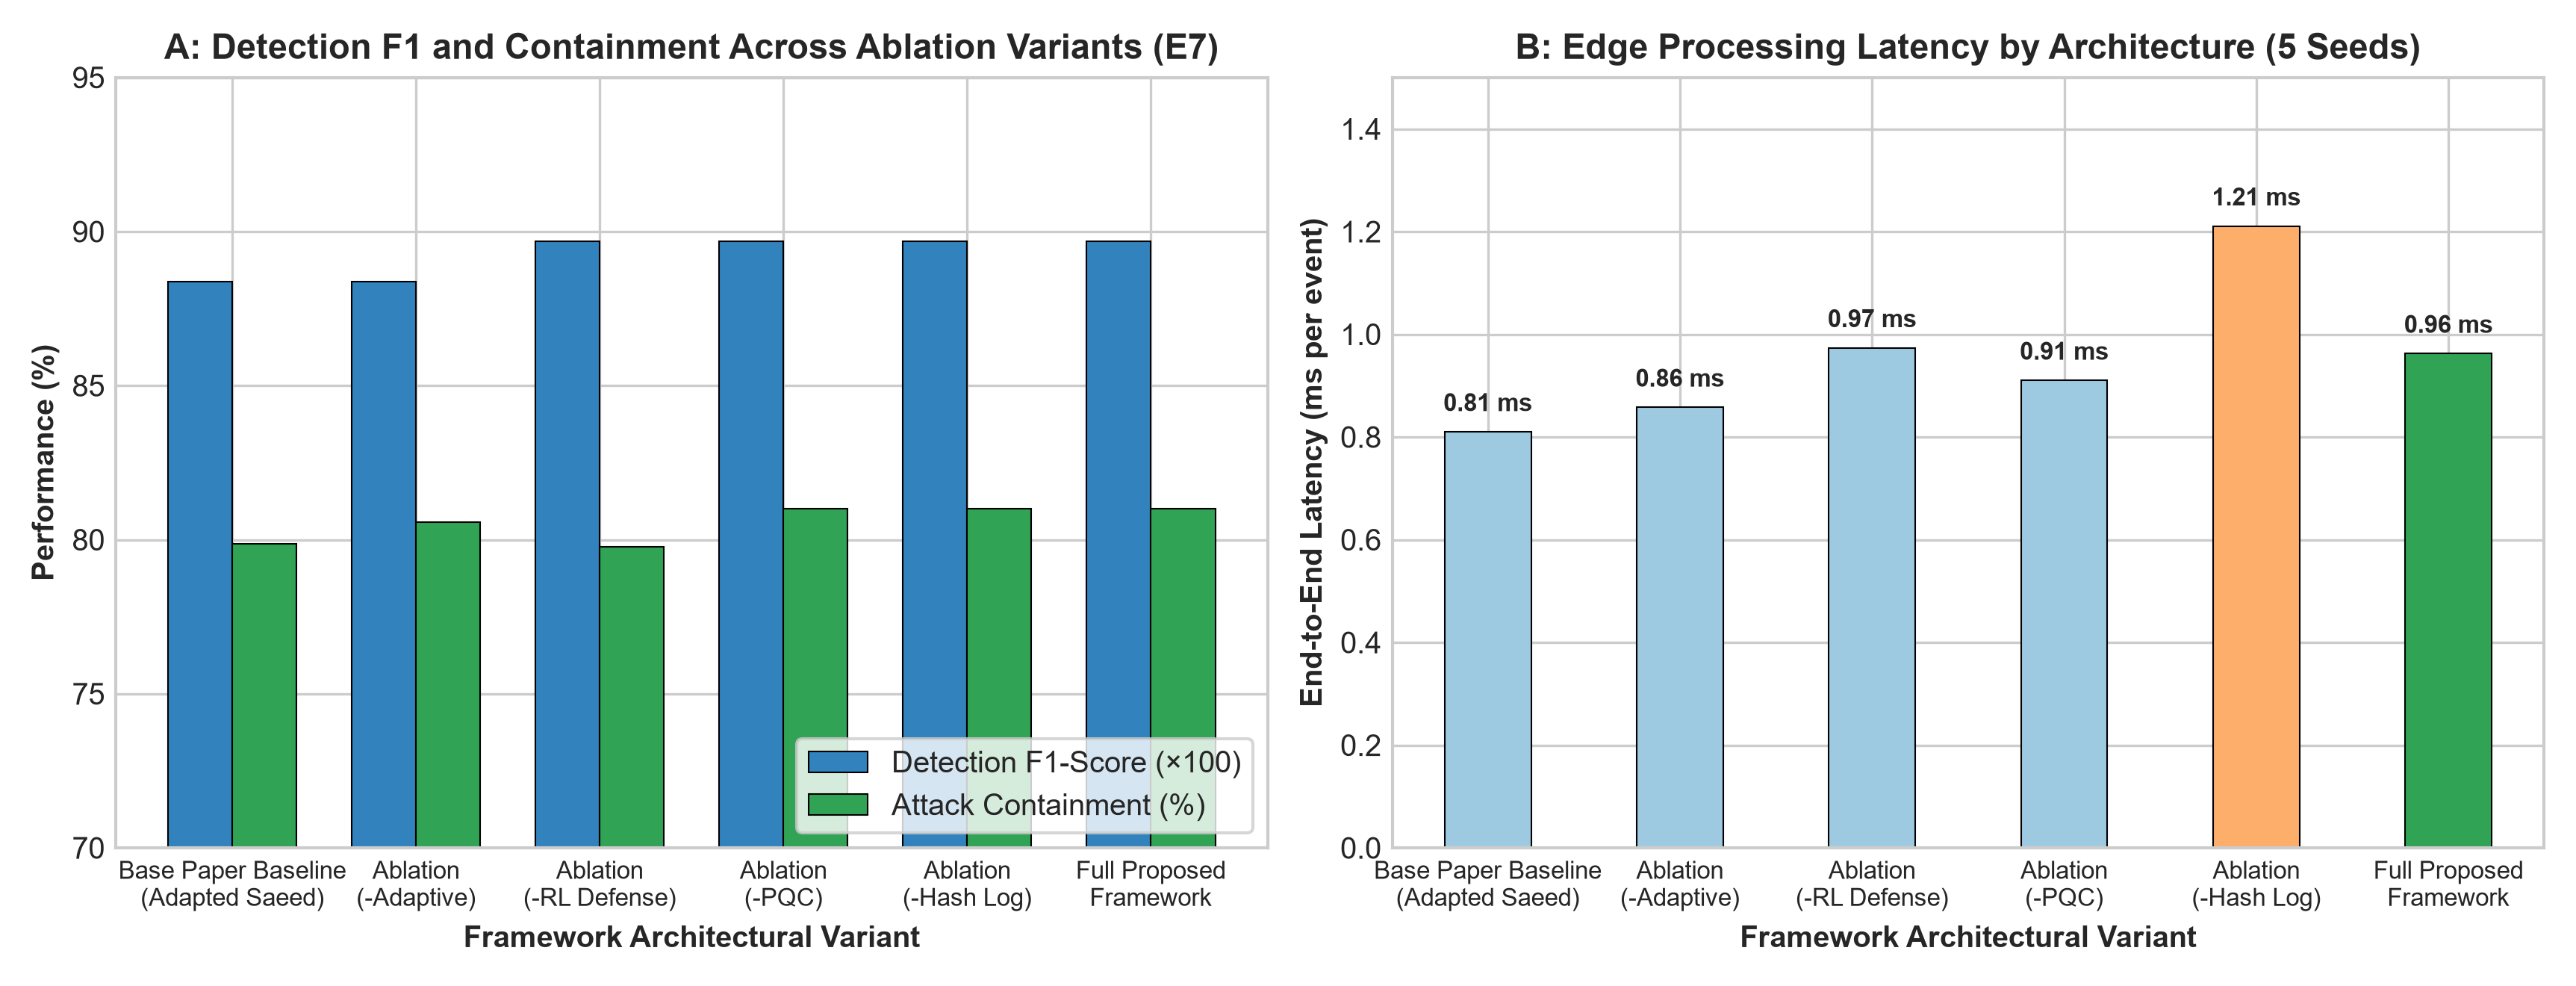
\includegraphics[width=0.48\textwidth]{figures/figure7_ablation_comparison.png}
\caption{Integrated Pipeline Component Ablation Comparison (Verified from Table VII Data).}
\label{fig:ablation_comp}
\end{figure}

\subsection{Multi-Dimensional Ablation Orthogonality}
A critical observation in Table~\ref{tab:e7_ablation} is that removing Post-Quantum Cryptography or Hash Chain Logging leaves the detection F1-score exactly unchanged ($0.8968 \pm 0.0013$). This invariance is expected due to the pipelined architecture: anomaly detection executes first, mapping telemetry features to reconstruction errors and binary decisions. Cryptographic encapsulation and append-only audit logging operate downstream on the resulting event record. Consequently, ablating cryptographic modules alters transport security and verifiable audit properties without modifying upstream feature loss or detection boundaries.

\subsection{Reconciliation of False Block Rates}
In standalone policy evaluation (Experiment E4), Tabular Q-Learning achieved a $0.00\%$ false block rate under idealized conditions. In contrast, in the integrated pipeline (Table~\ref{tab:e7_ablation}), the false block rate is $6.01\% \pm 1.52\%$. This difference reflects upstream detector noise propagation: Excluded EWMA thresholding has an empirical false positive rate of $\approx 13.6\%$ on bursty benign traffic. These false alarms increment the consecutive alert streak counter, causing the downstream Q-policy to escalate mitigation on subsequent benign flows. This realistic behavior highlights the necessity of end-to-end integrated evaluation over isolated micro-benchmarks.

\subsection{E8: Synthetic Feature Rate Stress Testing}
Table~\ref{tab:e8_stress} demonstrates the vulnerability of static 95th percentile thresholding under synthetic feature scaling applied to flow rate features (`Rate`, `Tot size`, `Variance`) of benign test samples. Under $2.0\times$ feature scaling, FPR explodes from $4.93\%$ to $27.33\%$ (+454.4% increase).

\textit{Operational Scope Disclosure}: In Experiment E8, synthetic scaling was applied strictly to rate features of benign test samples for Fixed 95th Percentile thresholding to evaluate sensitivity to burst telemetry. Excluded EWMA was evaluated on the base stream in Experiment E2 and was not re-evaluated under synthetic feature scaling in E8; threshold stability claims are strictly confined to the dynamic stream conditions tested in E2.

\begin{table}[h]
\centering
\caption{Static Threshold Sensitivity under Synthetic Rate Feature Scaling}
\label{tab:e8_stress}
\begin{tabular}{lcccc}
\toprule
Condition & Precision & Recall & F1-Score & FPR \\
\midrule
Fixed 95th Base ($1.0\times$) & $0.9893 \pm 0.0003$ & $0.8013 \pm 0.0022$ & $0.8854 \pm 0.0013$ & $0.0493 \pm 0.0013$ \\
Fixed 95th Stress ($1.5\times$) & $0.9796 \pm 0.0019$ & $0.8013 \pm 0.0022$ & $0.8815 \pm 0.0017$ & $0.0953 \pm 0.0092$ \\
Fixed 95th Stress ($2.0\times$) & $0.9436 \pm 0.0030$ & $0.8013 \pm 0.0022$ & $0.8666 \pm 0.0021$ & $\mathbf{0.2733 \pm 0.0152}$ \\
\bottomrule
\end{tabular}
\end{table}

\begin{figure}[h]
\centering
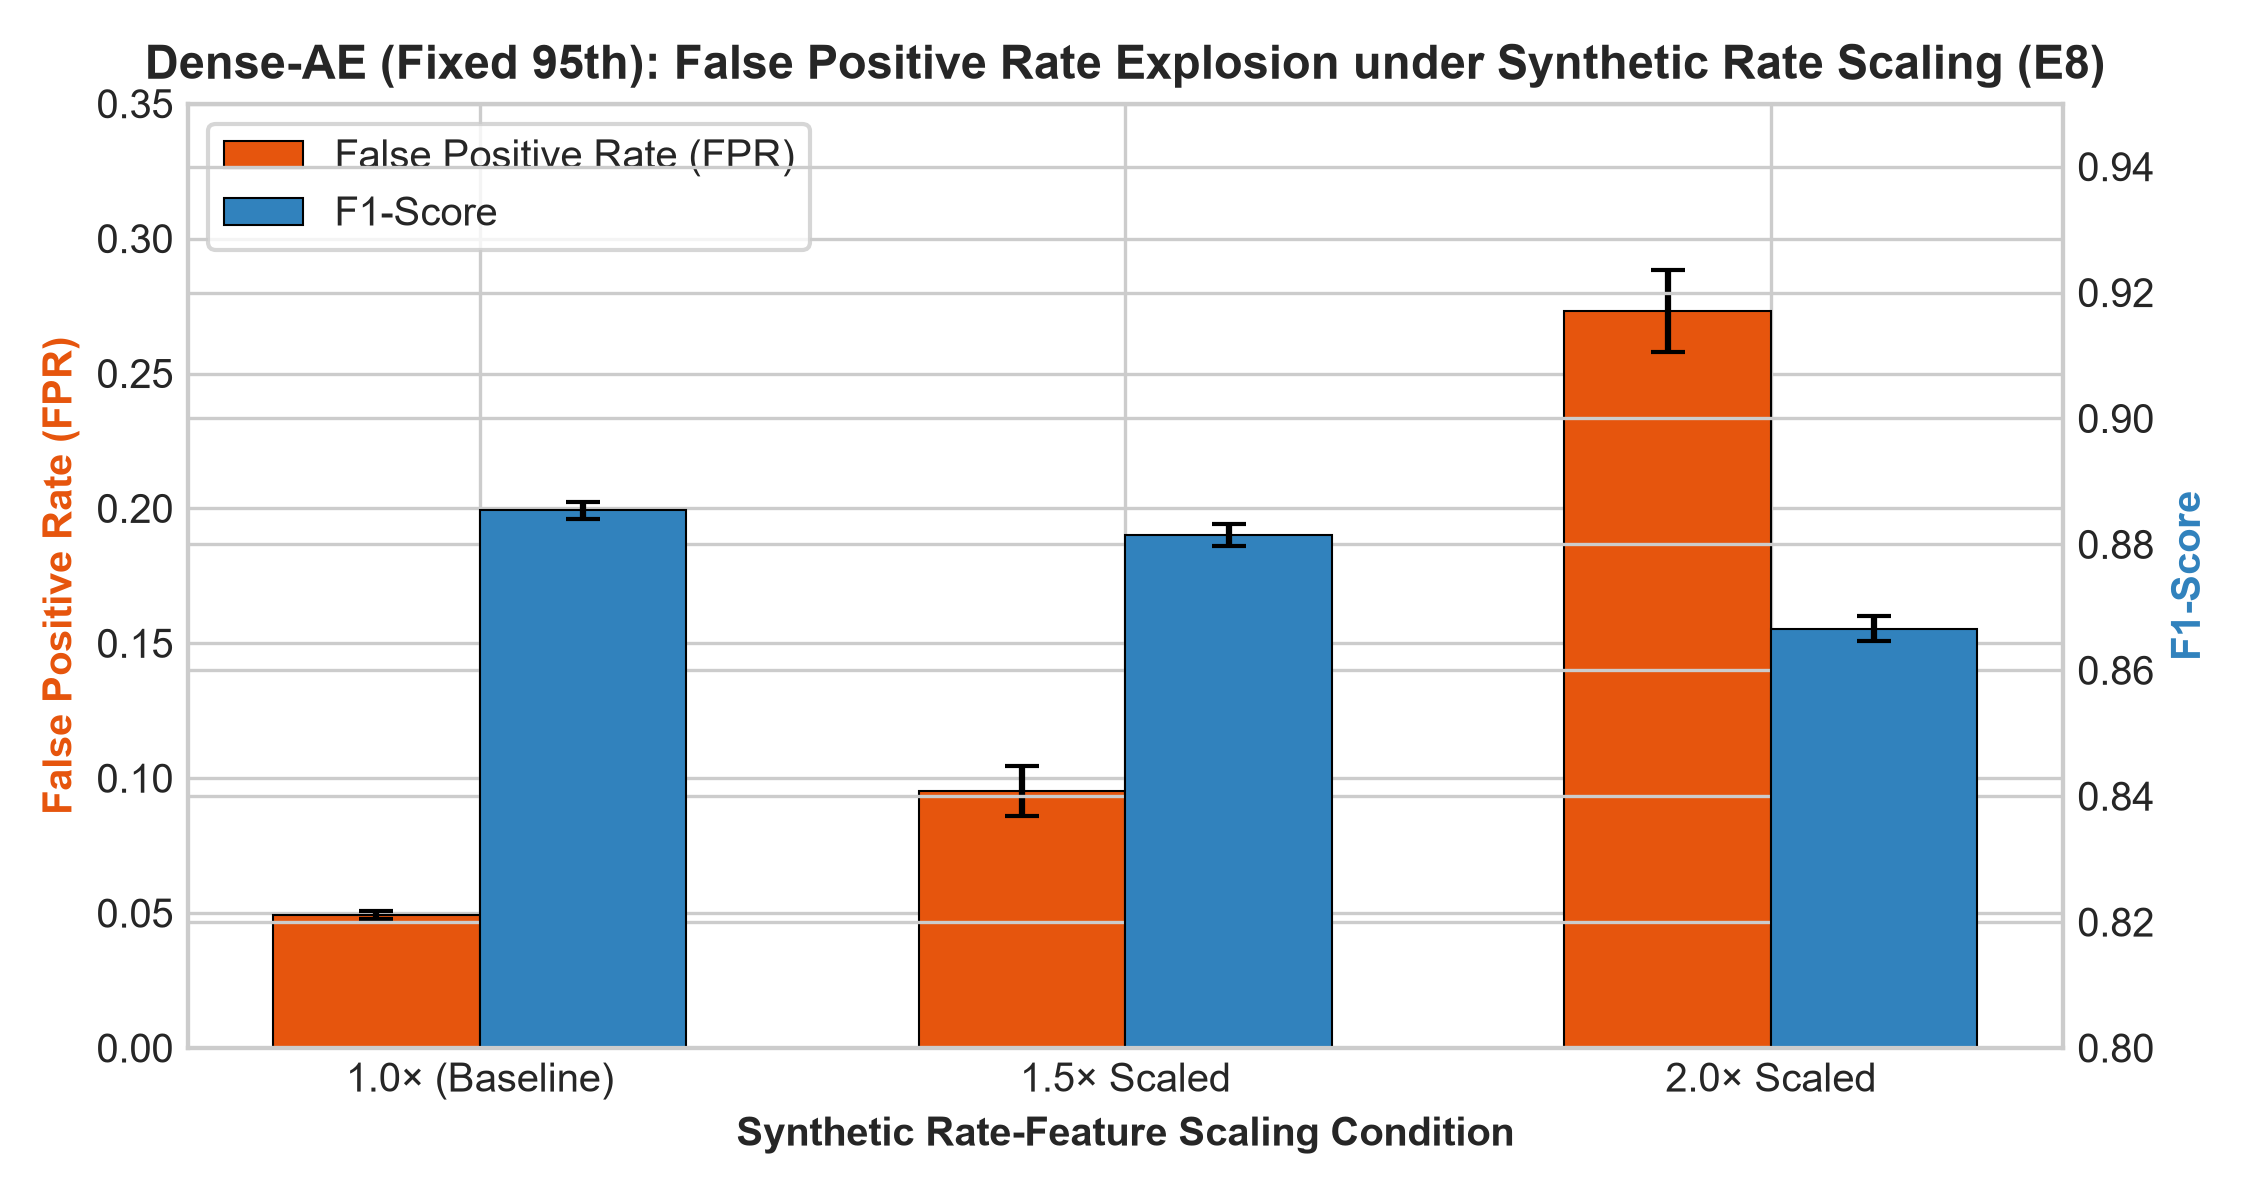
\includegraphics[width=0.48\textwidth]{figures/figure2_rate_stress_test.png}
\caption{False Positive Rate Explosion under Synthetic Rate Feature Scaling.}
\label{fig:rate_stress}
\end{figure}

\section{Statistical Analysis and Hypothesis Testing}
\label{sec:stats}
To establish rigorous empirical validity, Table~\ref{tab:stat_tests} presents paired $t$-tests, exact 95\% confidence intervals, Holm-Bonferroni adjusted $p$-values, and Cohen's $d$ effect sizes across the 5 evaluation seeds.

\begin{table}[h]
\centering
\caption{Hypothesis Testing and Effect Size across 5 Evaluation Seeds}
\label{tab:stat_tests}
\begin{tabular}{lcccc}
\toprule
Comparison & Mean Diff (95\% CI) & Paired $t$ & Adj. $p$ & Cohen's $d$ \\
\midrule
Excluded EWMA vs. Fixed 95th & $+0.0160$ [0.0147, 0.0173] & $33.81$ & $2.74\times 10^{-5}$ & $15.12$ \\
Fixed 95th vs. Fixed 99th & $+0.0195$ [0.0183, 0.0207] & $46.21$ & $1.05\times 10^{-5}$ & $20.67$ \\
Dense-AE vs. Isolation Forest & $+0.1089$ [0.0978, 0.1201] & $27.18$ & $5.45\times 10^{-5}$ & $12.16$ \\
Proposed vs. Baseline (Adapted) & $+0.0131$ [0.0113, 0.0149] & $19.89$ & $1.51\times 10^{-4}$ & $8.89$ \\
Proposed vs. Ablation (-Adapt) & $+0.0131$ [0.0113, 0.0149] & $19.89$ & $1.51\times 10^{-4}$ & $8.89$ \\
DQN vs. Tabular Q Containment & $+10.81\%$ [-3.90, 25.52] & $2.04$ & $0.2219$ & $0.91$ \\
Proposed vs. Ablation (-RL) & $+1.23\%$ [-2.28, 4.75] & $0.97$ & $0.3853$ & $0.44$ \\
\bottomrule
\end{tabular}
\end{table}

\section{Discussion}
\label{sec:discussion}
The empirical results reveal that dynamic thresholding is vital for balancing detection sensitivity against operational stability in IoT intrusion detection. While fixed percentile thresholds perform well on stationary traffic streams, they are fragile under traffic surges. Excluded EWMA prevents threshold inflation by separating detection from statistical estimation. In automated response, deep reinforcement learning provides a viable balance between attack containment and legitimate service preservation. Furthermore, NIST FIPS 203 ML-KEM-768 achieves practical sub-millisecond encryption for edge nodes, making post-quantum migration realistic for IoT infrastructure.

\section{Limitations and Threats to Validity}
\label{sec:limitations}
We explicitly disclose the following limitations:
\begin{enumerate}
    \item \textbf{Pre-Shuffled Dataset Origin}: Public CICIoT2023 records are pre-shuffled across captures. While our 5-seed duplicate-exclusion sensitivity test confirms that repeated feature vectors do not materially shift metrics ($\Delta\text{F1} \le -0.10\%$), device-level and capture-level independence cannot be established without raw physical network PCAP captures.
    \item \textbf{Local Storage Trust Boundary}: The append-only hash chain guarantees sequence integrity against unprivileged processes ($\mathcal{A}_{\text{proc}}$), but cannot prevent a root host adversary ($\mathcal{A}_{\text{root}}$) from rewriting local storage without external tip anchoring.
    \item \textbf{Hardware Deployment Scope}: Latency and throughput were measured on an AMD64 host edge gateway (3.40~GHz). Constrained microcontrollers (<100~MHz) require dedicated integer quantization and assembly optimization.
    \item \textbf{Synthetic Feature Scaling}: Experiment E8 applied analytical scaling to benign rate features rather than live network packet arrivals.
\end{enumerate}

\section{Reproducibility and Code Availability}
\label{sec:reproducibility}
To facilitate independent verification, the complete research codebase, model training scripts, evaluation notebooks, and raw result manifests are preserved in the accompanying reproducibility package. The complete regression test suite passes 30/30 tests in 26.91s (`results/final_submission_audit/test_report.xml`).

\textit{Public Code Repository Statement}: The source code, experiment scripts, reproducibility instructions, and raw experimental results are openly available at \url{https://github.com/Tanish-boop/AI-Driven-IoT-Cybersecurity-Framework-Research-}, with the evaluated codebase identified by its immutable release commit hash.

\section{Conclusion}
\label{sec:conclusion}
This study presented a benchmark of adaptive anomaly thresholding, un-contaminated reinforcement learning defense, standardized post-quantum cryptography, and cryptographic audit logging on CICIoT2023. Excluded EWMA resolves threshold inflation collapse (F1 = $0.9014 \pm 0.0018$), DQN achieves $71.26\%$ attack containment with $0.63\%$ false block rate, ML-KEM-768 provides sub-millisecond post-quantum transport security ($0.2758$~ms), and the full integrated framework achieves an end-to-end F1-Score of $0.8968 \pm 0.0013$ and $81.01\% \pm 2.83\%$ containment with sub-millisecond edge processing latency ($0.9626 \pm 0.6304$~ms per event, $1,436.2 \pm 759.5$~events/s throughput).

\section*{Acknowledgment}
The author acknowledges academic computing resources provided for this research.

\textit{IEEE Policy on Artificial Intelligence (AI) Use Disclosure}: Generative AI tools were utilized during manuscript preparation solely for formatting compliance, bibliographic verification, and LaTeX template synchronization. All experimental design, code execution, metric computation, and scientific interpretations were independently conceived, conducted, and verified by the author.

\bibliographystyle{IEEEtran}
\bibliography{references}

\begin{IEEEbiography}[{
\includegraphics[width=1in,height=1.25in,clip,keepaspectratio]{bullet.png}}]{Tanish Thakare}
is an independent researcher in cybersecurity and computer engineering. His research interests include Internet of Things (IoT) edge security, deep anomaly detection, adaptive thresholding mechanisms, reinforcement learning for autonomous defense mitigation, and post-quantum cryptographic protocols.
\end{IEEEbiography}

\EOD

\end{document}
